\documentclass{article}

\date{\today} 
 %\setlength{\parskip}{1em}
% \usepackage[round, sort, comma]{natbib}
% \setcitestyle{notesep={, },round,aysep={},yysep={,}}

%\setlength{\parindent}{0pt}

% \usepackage[authordate,strict,backend=bibtex8,babel=other, doi=false, url=false, isbn=false, uniquename=false, maxcitenames = 2, uniquelist=false,%
% bibencoding=inputenc, natbib]{biblatex-chicago}
%\usepackage[authordate, backend=biber, doi=false, url=false, isbn=false, uniquename=false, maxcitenames = 2, uniquelist=false, natbib]{biblatex-chicago}



% ---------------------------------------
%   REFERENCES
% ---------------------------------------
\usepackage{natbib} %[round, sort, comma]{natbib}
  \bibpunct[: ]{(}{)}{;}{a}{}{,}
%\usepackage[nottoc,numbib]{tocbibind} % numbers bib. in table of contents


% ---------------------------------------
%   MARGINS AND SPACING
% ---------------------------------------
\usepackage[margin=1in]{geometry} 
\usepackage{setspace} % line spacing


% ---------------------------------------
%   TABLES AND FIGURES
% ---------------------------------------
\usepackage{graphicx} % input graphics
\graphicspath{ {./Figs/} }

\usepackage{float} % float parameters
\usepackage{placeins} % \FloatBarrier: prevent floats spilling across sections
\usepackage{subcaption} % subfloats with individual captions
\usepackage{multirow} % multicolumn and multirow
\usepackage{booktabs} %? for toprule, midrule etc
\usepackage{dcolumn} % decimal-aligned columns

\usepackage{tikz}
\usetikzlibrary{positioning}
\usetikzlibrary{shapes.geometric}
\usetikzlibrary[patterns]

% ---------------------------------------
%   MATH
% ---------------------------------------
\usepackage{amsmath}
%  Math symbols (depends on whether you customize typeface)
%  \usepackage{amsfonts}
%  \usepackage{mathrsfs}
\usepackage{amssymb}
  %  \newcommand{\E}{\mathrm{E}}
  %  \newcommand{\Var}{\mathrm{Var}}
  %  \newcommand{\Cov}{\mathrm{Cov}}
  %  \newcommand{\plim}{\mathrm{plim}}
  %  \renewcommand{\L}{\mathcal{L}}
  %  \renewcommand{\d}{\mathrm{d}}
  %  \newcommand{\R}{\mathbb{R}}


% ---------------------------------------
%   TYPEFACE AND TEXT STYLES
% ---------------------------------------


% \usepackage{fontenc} 
% advisable to include for nitty-gritty details
% (ligatures, kerning & other typographical things)

% \usepackage[usenames, dvipsnames]{xcolor} % extra colors
\usepackage{hyperref} % hyperlinks
   \hypersetup{
     colorlinks = true, 
     citecolor = black, 
     linkcolor = blue,
     urlcolor = blue}

\usepackage{comment} % provides {comment} environment
\usepackage{enumitem} % allows [nosep] option for lists

\usepackage{endnotes}

\makeatletter
\renewcommand\@makeenmark{%
  \textsuperscript{\normalfont\textcolor{blue}{\@theenmark}}%
}
\newcommand{\uncolormarkers}{%
  \renewcommand\@makeenmark{%
    \textsuperscript{\normalfont\@theenmark}%
  }%
}
\makeatother


\newcommand{\exclude}[1]{\StopSearching ##1\StartSearching}

\usepackage{ragged2e}

% \usepackage{figcaps}
% \setlength{\parskip}{1em}
\title{Why Do Agencies (sometimes) Get So Much Mail? \\
Lobbying coalitions, mass comments, and political information in bureaucratic policymaking}

\author{Devin Judge-Lord \\ JudgeLord@Wisc.edu}

% FOR DAVE: %%%%%%%%%%%%%%%%%%%%%%%%%%%
% \let\footnote=\endnote
% \renewcommand{\footnotesize}{\normal}
%%%%%%%%%%%%%%%%%%%%%%%%%%%%%%%%%%%%%%%
\begin{document}

% FOR DAVE: %%%%%%%%%%%%%%%%%%%%%%%%%%
% \Large
% \RaggedRight
%%%%%%%%%%%%%%%%%%%%%%%%%%%%%%%%%%%%%%
\maketitle

\centering THIS DRAFT WAS PREPARED FOR APW 2019. THE MOST RECENT DRAFT IS \href{https://github.com/judgelord/dissertation/raw/master/whyMail.pdf}{HERE}.

\abstract{Scholars of bureaucratic policymaking have focused on the sophisticated lobbying efforts of powerful interest groups. Yet agencies occasionally receive thousands or even millions of comments from ordinary people. Why? Why do individuals comment when they seemingly have no new information to offer and no power to influence decisions? Who inspires them and to what end? How, if at all, should scholars incorporate mass commenting into models of bureaucratic policymaking? I argue that mass commenting produces political information about the coalition that mobilized it. To link individual comments to the more sophisticated lobbying efforts they support, I use text reuse and topic models to identify clusters of similar comments, reflecting formal and informal coalitions. I also classify different types of supporters. Using these new measures of political mobilization and engagement in agency rulemaking, I identify the conditions under which mass comment campaigns occur and produce different types of politically-relevant information.}


\newpage
% \tableofcontents

\newpage
\section*{Note to reader:}
Thank you so much for reading this very rough draft. For context, this is the first chapter developing concepts and measures of public engagement in agency rulemaking that will be used in the following empirical chapters. The methods are under construction, and the limited findings are tentative.
%In the dissertation, I argue that mass participation results from interest groups' strategic choices. When lobbying organizations have an opportunity to shape policy, the resources to mobilize, and broader support than their opposition, outside lobbying (``going public'') may produce valuable, politically-relevant information. Depending on how agencies process political information, outside lobbying may %be a plausible strategy for organizations to 
%influence policy, both directly and indirectly.
%For example, those lobbying in rulemaking often make dubious claims to represent broad segments of the public. Mobilizing a large number of people may directly support such claims.
%Indirectly, it may alert elected officials to political risks and opportunities, affecting oversight behavior. % and thus shifting bureaucrats' relationships with their political principals. % It remains to be seen if conditions under which this is plausible ever occur and, if so, if mass engagement does indeed influence policy. 

The broader project aims to better understand the role of ordinary people in bureaucratic policymaking. 
I develop theories of why mass engagement occurs and how it may affect policy. To assess these theories, I tackle three related empirical questions: (1) Why does it occur?; (2) How does it affect the oversight behaviors of agencies' political principals?; and %These questions drive two initial empirical chapters.
(3)  Does mass engagement in bureaucratic policymaking affect policy?
% I then use my new measures of the political information that lobbying coalitions create by going public to test whether mass engagement explains variation in agency rulemaking and rules.% But first, I must develop a measure of ``going public.'' % and why it occurs.

\paragraph{Part 1. Why do agencies (occasionally) get so much mail?} %: Lobbying coalitions, mass comments, and political information in bureaucratic policymaking
% Scholars of bureaucratic policymaking have focused on the sophisticated lobbying efforts of powerful interest groups. Yet agencies occasionally receive thousands or even millions of comments from ordinary people. Why? Why do individuals comment when they seemingly have no new information to offer and no power to influence decisions? Who inspires them and to what end? How, if at all, should scholars incorporate mass commenting into models of bureaucratic policymaking? I argue that mass commenting produces political information about the coalition that mobilized it. 
% QUESTION 1\textbf{Puzzle:} 
Why do some rules receive many comments from ordinary people and some do not?
% Why do people comment on draft policies when they seem to have no new information to offer and no power to influence decisions? Who inspires them and to what end? 
% THEORY AND METHODS 1
% Answering this question requires a theory explaining variation in mass engagement. 
The literature suggests two possible explanations for variation in mass engagement; groups may leverage public support as a lobbying resources (``grass roots'' mobilization) or groups with more resources may leverage those resources into impression of public support (sometimes called ``astro-turf'').
%Using new measures of public engagement in agency rulemaking, I identify the conditions under which it occurs and produces different politically-relevant information. 
% The dependent variable is the number of people engaged.
I theorize that public support explains variation in mass engagement. That is, unlike other forms of lobbying, it not primarily driven by groups with more resources. Specifically, I anticipate three patterns:
(1) When a coalition is disadvantaged in insider politics but as more public support than opposing coalitions, they are more likely to ``go public'' to bolster their lobbying effort (assuming they have the resources to do so). More public support yields more engagement, more effort per participant, and contagion beyond those mobilized directly. (2) Coalitions with less support may ``counter-mobilize'' with proportionally smaller results. That is, groups with more resources but less public support only mobilize when their opponents do so. (3) Finally, coalitions may mobilize for reasons unrelated to the policy at hand, yielding significant mass engagement but without a corresponding insider lobbying effort. 
Because the vast majority of comments are inspired by interest-group campaigns, finding their cause requires a method to link comments to the lobbying coalitions that mobilized them.  
To link individual comments to the more sophisticated lobbying efforts they support, I use text reuse and clustering methods to capture formal and informal coalitions.
Measures of mass engagement include 
%(1) total public comments, % $\sim$ zero-inflated negative binomial; 
(1) comments per coalition, % $\sim$ negative binomial; 
(2) effort per comment, % $\sim$ truncated normal; 
(3) share of comments per coalition mobilized indirectly (i.e. the potential for conflict spread).
With measures, I test whether variation in engagement explains variation in oversight behavior (part 2) and policy outcomes (part 3).
% (4) type of campaign. % $\sim$ multinomial. 
%Model 1 is one observation per rule. Models 2-4 are one observation per coalition per rule. Explanatory variables include agency alignment with Congress and the president (models 1-4), coalition alignment and unity (models 2-4), whether a coalition is driven more by public or private interests (models 2-3).%, part of the DV in model 4).

%\paragraph{Step 2. Are elected officials more or less likely to engage after mass public engagement?} 
\paragraph{Part 2. Does mass engagement affect political oversight?} The political information signaled by mass engagement may serve as a ``fire alarm,'' altering principals to oversight opportunities or ``warning signs'' altering them to political risks.
When a coalition mobilizes successfully, %especially if it generates a perceived consensus in expressed public sentiments, 
elected officials ought to be more likely to engage on their behalf and less likely to engage against them.
% This suggests an addendum to Hall and Miler's (2008) finding that members are more likely to engage in rulemaking when they have been lobbied by a like-minded interest group.
% When interest groups lobby elected officials to engage in rulemaking, they may be more likely to engage when aligned with most commenters than when opposed.
% If politicians learn from political information, they will be even more likely to engage when lobbied by a coalition that includes a public interest group's with a large mass-comment campaign, and less likely when lobbied by a coalition dominated by private interests opposed by a mass comment campaign. 
% MEASUREMENT  2
To assess these hypotheses, I count the number of times Members of Congress engage the agency before, during, and after comment periods on rules where lobbying organizations did and did not go public. I then use text analysis to compare legislators' sentiments and rhetoric to that used by each coalition.
% Similarly, I asses the involvement of presidential appointees and the President's Office of Management and Budget before and after public comment, again comparing rules that were and were not targeted by a campaign (a difference-in-difference). 
% As a validity check, I also look for remarks by elected officials and judges on the level of public engagement.
Dependent variables include 
(1) the number of comments from Members of Congress on the rule %(total, those mentioning mass comments, and those mentioning organizations in the coalition), %All  $\sim$ zero-inflated negative binomial. 
(2) the share of supportive congressional comments, %  $\sim$  beta. 
(3) the similarity of words in comments from the coalition and Members of Congress. 

\paragraph{Part 3. Does mass engagement affect rulemaking and rules?} 
I theorize that the effects of political information on policy depend on the extent to which the strategic environment allows change and how political information is processed, both directly within agencies and indirectly through other actors (e.g. Members of Congress) whose appraisals matter to bureaucrats.
The main dependent variable is change in the rule text.
%Different inputs may yield different results: 
I systematically identify changes between draft and final rules, parse these differences to identify meaningful policy changes, and compare them to demands raised in comments to measure which coalition got their desired outcomes.% However, assessing policy change is difficult. Thus, I also use other measures of agency responses to lobbying efforts. 

\doublespace
% \section*{Summary}
% 
%\paragraph{Summary:} 
% This dissertation is about ordinary people's input on policies made by bureaucrats. 
% % People may believe that their voices matter, but it is unclear if they do. % or ought to. 
% I make three main contributions. First, drawing on scholarship on interest group behavior, social movements, and lobbying, I suggest three distinct reasons for groups to mobilize ordinary people. Each logic suggests a different pattern of mass engagement, and I analyze millions of public comments on thousands of agency rules to develop the first systematic measures of mass engagement in bureaucratic policymaking. Second, building on theories of political oversight, I theorize that mass public engagement in bureaucratic policymaking may alert elected officials to political opportunities and risks. I assess this argument by analyzing correspondence between Members of Congress and bureaucrats on proposed rules. Third, I integrate these contributions on interest group lobbying and oversight into a broader theory of the potential for mass mobilization to affect policy. I argue that there are four broad causal mechanisms by which lobbying may affect bureaucrats' decisions. Political scientists have thus far focused on the power of technical information where insider lobbying is most likely to matter and outside lobbying is least likely to matter and have thus largely overlooked mass engagement. This gap suggests that incorporating theories of social movement influence may advance bureaucratic politics scholarship and that bureaucratic politics may be a fruitful empirical ground for exploring social movement theories. I use my new measures of mass engagement to assess the effect of political information on bureaucratic policymaking. Finally, two chapters examine the four causal mechanisms I suggest through a case study of the environmental justice movement and a study of rules where organizations randomly select lobbying strategies.

%I theorize that mass engagement may, in limited circumstances, influence bureaucrats by shifting their incentives or evoking powerful norms. Using my new measures to assess these mechanisms, 
%I show how various parts of the U.S. government respond to public input.  %aims to understand the effects of public attention on executive-branch policymaking.

\paragraph{Motivation:} Leading models of influence in bureaucratic policymaking focus on two key political forces: sophisticated interest group lobbying and political oversight. 
As bureaucrats learn about policy problems and balance interest-group demands, public comment processes allow lobbying organizations to provide useful technical information and inform decisionmakers of their preferences on draft policies. 
Agencies may then update policy positions within constraints imposed by their political principals.

While this may describe most cases of bureaucratic policymaking, these models do not explain or account for the contentious politics that occasionally inspire millions of ordinary people to respond to calls for public input on draft agency policies. Mass engagement in bureaucratic policymaking has thus largely been ignored by political scientists, leaving a weak empirical base for normative and prescriptive work. 
Like other forms of mass political participation, such as protests and letter writing campaigns, 
mass public comments on draft agency rules provide no new technical information. %In this sense, they are not useful. 
Nor do they wield any formal authority to reward or sanction bureaucrats, as comments from a Members of Congress might. 
The number on each side, be it ten or ten million, has no legal import for an agency's response. 
% Policymakers may very well pay no attention to them. 
%Instead, scholars focus on the sophisticated lobbying efforts of powerful interest groups, whose role in shaping policy has been theoretically developed and empirically tested.
% If our models and conventional wisdom is correct, why do
Yet agencies occasionally receive input from a large number of ordinary people. %Why? 
How, if at all, should scholars incorporate mass engagement into models of bureaucratic policymaking? 

I argue that mass engagement results from interest groups' strategic choices. When lobbying organizations have an opportunity to shape policy, resources to mobilize, and broader support than their opposition, outside lobbying (``going public'') may produce valuable, politically-relevant information. Depending on how agencies process political information, outside lobbying may %be a plausible strategy for organizations to 
influence policy, both directly and indirectly.
For example, those lobbying in rulemaking often make suspect claims to represent broad segments of the public. Mobilizing a large number of people may directly support such claims.
Indirectly, it may alert elected officials to political risks and opportunities, affecting oversight behavior. % and thus shifting bureaucrats' relationships with their political principals. % It remains to be seen if conditions under which this is plausible ever occur and, if so, if mass engagement does indeed influence policy. 

Does mass engagement in bureaucratic policymaking affect policy? This question drives my project. However, two questions must be answered first: (1) Why does it occur? and (2) How does it affect the oversight behaviors of agencies' political principals? These questions drive two initial empirical chapters.
I then use my new measures of the political information that lobbying coalitions create by going public to test whether mass engagement explains variation agency rulemaking and rules.% But first, I must develop a measure of ``going public.'' % and why it occurs.

\paragraph{Step 1. Why do agencies (occasionally) get so much mail?} %: Lobbying coalitions, mass comments, and political information in bureaucratic policymaking
% Scholars of bureaucratic policymaking have focused on the sophisticated lobbying efforts of powerful interest groups. Yet agencies occasionally receive thousands or even millions of comments from ordinary people. Why? Why do individuals comment when they seemingly have no new information to offer and no power to influence decisions? Who inspires them and to what end? How, if at all, should scholars incorporate mass commenting into models of bureaucratic policymaking? I argue that mass commenting produces political information about the coalition that mobilized it. 
% QUESTION 1\textbf{Puzzle:} 
Why do people comment on draft policies when they seem to have no new information to offer and no power to influence decisions? Who inspires them and to what end? 
% THEORY AND METHODS 1
Answering these questions requires a theory explaining variation in mass engagement and method to link comments to the lobbying coalitions that mobilized them.  
To link individual comments to the more sophisticated lobbying efforts they support, I use text reuse and Bayesian classifiers to identify clusters of similar comments, reflecting formal and informal coalitions.
%Using new measures of public engagement in agency rulemaking, I identify the conditions under which it occurs and produces different politically-relevant information. 
% The dependent variable is the number of people engaged.
I argue that activists' resources, opportunities, and public support explain variation in mass engagement %, which I measure in several ways. 
and that it will fit one of three patterns:
(1) Coalitions will ``go public'' when they are disadvantaged in insider politics but have more support than opposing coalitions. More public support yields more engagement, more effort per comment, and contagion beyond those mobilized directly. (2) Coalitions with less support may ``counter-mobilize'' with smaller effects. (3) Finally, coalitions may mobilize for reasons unrelated to the policy at hand, yielding similar mass engagement but with little sophisticated lobbying. 
Measures of mass engagement include 
%(1) total public comments, % $\sim$ zero-inflated negative binomial; 
(1) comments per coalition, % $\sim$ negative binomial; 
(2) effort per comment, % $\sim$ truncated normal; 
(3) share of comments per coalition mobilized indirectly (i.e. the potential for conflict spread).
Next, I test whether variation in engagement explains variation in oversight behavior (step 2) and policy outcomes (step 3).
% (4) type of campaign. % $\sim$ multinomial. 
%Model 1 is one observation per rule. Models 2-4 are one observation per coalition per rule. Explanatory variables include agency alignment with Congress and the president (models 1-4), coalition alignment and unity (models 2-4), whether a coalition is driven more by public or private interests (models 2-3).%, part of the DV in model 4).

%\paragraph{Step 2. Are elected officials more or less likely to engage after mass public engagement?} 
\paragraph{Step 2. Does mass engagement affect political oversight?} The political information signaled by mass engagement may serve as a ``fire alarm,'' altering principals to oversight opportunities or a ``warning signs'' altering them to political risks.
When a coalition goes public, %especially if it generates a perceived consensus in expressed public sentiments, 
principals ought to be more likely to engage on their behalf and less likely to engage against them.
% This suggests an addendum to Hall and Miler's (2008) finding that members are more likely to engage in rulemaking when they have been lobbied by a like-minded interest group.
% When interest groups lobby elected officials to engage in rulemaking, they may be more likely to engage when aligned with most commenters than when opposed.
% If politicians learn from political information, they will be even more likely to engage when lobbied by a coalition that includes a public interest group's with a large mass-comment campaign, and less likely when lobbied by a coalition dominated by private interests opposed by a mass comment campaign. 
% MEASUREMENT  2
To assess these hypotheses, I count the number of times Members of Congress engage the agency before, during, and after comment periods on rules where lobbying organizations did and did not go public. I then use text analysis to compare legislators' sentiments and rhetoric to that used by each coalition.
% Similarly, I asses the involvement of presidential appointees and the President's Office of Management and Budget before and after public comment, again comparing rules that were and were not targeted by a campaign (a difference-in-difference). 
% As a validity check, I also look for remarks by elected officials and judges on the level of public engagement.
Dependent variables include 
(1) the number of comments from Members of Congress on the rule %(total, those mentioning mass comments, and those mentioning organizations in the coalition), %All  $\sim$ zero-inflated negative binomial. 
(2) the share of supportive congressional comments, %  $\sim$  beta. 
(3) the similarity of words in comments from the coalition and Members of Congress. 
% Models 1 and 2 are one observation per coalition per rule. Model 3 is one observation per comment from a Member of Congress. Explanatory variables of interest are the dependent variables from step 1 (how many and what types of comments--i.e. variation in political information).% In addition to cross-sectional analysis, I use a difference-in-difference design within members on rules where groups do and do not go public.

%I examine the relationship between mass engagement and another key variable in agency decisions, political oversight. % other key features of agencies' decisionmaking environments. 
% Do mass comment campaigns indicate that elected officials will be more involved in a rulemaking? 
% Do they indicate a greater chance of a rule being challenged or overturned in court?
% Dependent variables include political principals' attention, positions, and rhetoric, which I measure several ways across rules and within policy areas before and after mobilization campaigns.
% THEORY 2
% Accountability to Congress, the president, and courts have long been central concerns for bureaucracy scholars \citep{Wilson1989}. 
 % Elected officials, political appointees, and judges may also see it as their job to hold agencies accountable to the public will. On the other hand, elected officials often serve private interests,  such as campaign donors, especially when there is little risk of being held publicly accountable themselves.






% QUESTION 3 
% Are changes in rulemaking and rules more likely after mass engagement?
\paragraph{Step 3. Does mass engagement affect rulemaking and rules?} I theorize that the effects of political information on policy depend on the extent to which the strategic environment allows change and how political information is processed, both directly within agencies and indirectly through other actors (e.g. Members of Congress) whose appraisals matter to bureaucrats.
The main dependent variable is change in the rule text.
%Different inputs may yield different results: 
I will systemically identify changes between draft and final rules, parse these differences to identify meaningful policy changes, and compare them to demands raised in comments to measure which coalition got their way. However, assessing policy change is difficult. Thus, I will also use other measures of agency responses to lobbying efforts. %For example, agencies may speed up or delay finalizing rules. They write lengthy justifications of their decisions in response to some demands but not others. They may or may not extend the comment period.


% \paragraph{Step 4. Causal mechanisms:} How might mass engagement matter?
% A lobbying effort can generate new information, re-frame information, or reshape the political context of a decision. Agency staff may update their beliefs in response to new information or framing. Activists can also reshape agency policymakers’ strategic environment by drawing in or scaring off other actors, especially elected officials. 

% \textbf{Strategic calculations:} 
% New information may affect bureaucrats' decisions directly or indirectly. New scientific or legal information spurs revision of calculations about cost and benefits or the likelihood of being reversed in court. New political information spurs bureaucrats to update their beliefs about levels of support among segments of the public or their elected representatives and thus about the likely political consequences of a decision.
% % Reshaping strategic incentives may shift how rulewriters weigh commenter demands.

% % NORMATIVE FRAMING / INFO PROCESSING 
% \textbf{Information processing and normative evaluations:} 
% In addition to strategic calculations, mass engagement may shift how information is processed and evaluated, both institutionally and cognitively.
% Institutionally, higher comment volume may engage a larger and more politically-oriented set of staff and consultants. Cognitively, expanding the scope of conflict highlights the political aspects of a decision, perhaps mobilizing cognition focused more on norms of public service or partisan ideology than on strategic or technical rationality. In both cases, campaigns re-frame decisions as political and provide information that is especially relevant if processed through such a frame.
% The effects of political information on bureaucrats' normative evaluations may be
% direct---the weight that norms of direct democracy give to limited public input---or 
% indirect---the weight that norms of accountability give to elected officials' input.

% %\textbf{Indirect influence through elected officials:} 
% %Campaigns  do more than reveal latent political information; they mobilize both members of the public and elected officials to take positions on issues they may have never previously considered, thus creating new relevant political information for bureaucrats. 
% %Movements help to shape the political space in which they operate’ (Gamson and Meyer 1996, p. 289).
% %The result of thinking differently about a decision may be a shift in how the agency evaluates or weights commenter demands.

\textbf{Assessing causal mechanisms:} While it may be impossible to causally identify or attribute effects to normative or strategic mechanisms, 
a focus on political information suggests places to look for influence in rulemaking. For example, if Members of Congress are not more likely to voice support for a coalition that goes public, this would be evidence against any indirect mechanism via congressional oversight.

To supplement the core design above, the two additional chapters explore historical and experimental case studies. My historical case is the environmental justice movement, relying on all rules where ``environmental justice'' is raised in the comments and quantitative and qualitative assessment of agency responses. I find that responsiveness varies across agencies. My experimental cases will be rules selected by organizations that have agreed to randomly assign specific targets of their mass comment campaigns. In exchange, I will use the methods outlined above to estimate the effects of their interventions. 

% \paragraph{Conclusion:} This research will add to our understanding of how bureaucratic policymaking fits with the practice of democracy.
% If input solicited from ordinary people has little effect on policy outcomes, directly or indirectly, it may be best understood as providing a veneer of democratic legitimacy on an essentially technocratic and/or elite-driven process.
% If public input does shape agency decisions, a new research program will be needed to investigate who exactly these campaigns mobilize and represent.

% \end{document} % NO SOURCES BEFORE THIS POINT

\newpage
\section{Introduction} \label{intro}

Paticipatory processes like public comment periods, where government agencies must solicit public input on draft policies, are said to provide political oversight opportunities \citep{Balla1998, Mccubbins1984}, democratic legitimacy \citep{Croley2003, Rosenbloom2003}, and new technical information \citep{Yackee2006JPART, Nelson2012}. %\footnote{These various goals are evident in the Proposed Recommendation on Public Engagement in Rulemaking from the Administrative Conference of the United States, which asserts that ``The opportunity for public engagement is vital to the rulemaking process, permitting agencies to obtain more comprehensive information, enhance the legitimacy and accountability of their decisions, and enhance public support for their rules'' \citep{ACUS2018}.}
%Public comment periods are purported to simultaneously produce technical information, accountability to elected officials, and responsiveness to public demands.
While recent scholarship on agency policymaking has shed light on the sophisticated lobbying by businesses and political insiders, we know surprisingly little about the vast majority of public comments which are submitted by ordinary people as part of public pressure campaigns.\footnote{As I show elsewhere \citep{Judge-Lord2019}, most comments submitted to regulations.gov are form comments, more akin to petition signatures than sophisticated lobbying. Indeed, aproximately 40 million out of 50 million (80\%) of these public comments mobilized by just 100 advocacy organizations.}
Activists frequently target agency policymaking with letter-writing campaigns, petitions, protests, and mobilizing people to attend hearings, all classic examples of ``civic engagement'' \citep{Verba1987}. Yet civic engagement remains poorly understood in the context of bureaucratic policymaking.

These occasional bursts of civic engagement in bureaucratic policymaking raise practical and theoretical questions for the practice of democracy.\footnote{In 2018, the Administrative Conference of the United States (ACUS) identified mass commenting as a top issue in administrative law. In their report to ACUS, \citet{SantAmbrogio2018} conclude, ``The `mass comments' occasionally submitted in great volume in highly salient rulemakings are one of the more vexing challenges facing agencies in recent years. Mass comments are typically the result of orchestrated campaigns by advocacy groups to persuade members or other like-minded individuals to express support for or opposition to an agency's proposed rule.'' 
Mass comment campaigns are known to drive significant participation of ordinary people in Environmental Protection Agency rulemaking \citep{Judge-Lord2019, Potter2017, Balla2018}. \citet{Cuellar2005}, who examines public input on three rules, finds that ordinary people made up the majority of commenters demonstrating ``demand among the mass public for a seat at the table in the regulatory process.'' } 
%To date, administrative law scholars have focused on practical and normative questions, much of this analysis depends 
These questions, in turn, hinge on unanswered empirical questions: Do these campaigns affect policy? If so, by what mechanisms? Existing research finds that commenters believe their comments matter \citep{Yackee2015JPART} and that the number of public comments varies across agencies and policy processes \citep{Judge-Lord2019, Libgober2018, Moore2017},
% and policy change is related to the number of comments in sample of nine rules \citep{Shapiro2008}, 
but the relationship between the scale of public engagment and policy change remains untested. 

To address this gap, I assess the relationship between the number of public comments and the amount of change between draft and final policy texts. Next, I assess the relationship between the number of people mobilized by each campaign and whether the campaign acheivied its policy goals. Finally, I theorize and test four mechanisms by which public input may affect bureaucratic policymaking. Each mechanism involves a distinct type of information that pressure campaigns may relay to policymakers: technical information, information about the likelihood of political consequences, information about the preferences of elected officials, or information about the preferences of the attentive public. Because scholarship on bureaucratic policymaking has focused on the power of technical information, where insider lobbying is most likely to matter and where outside strategies are least likely to matter, political scientists have largely overlooked mass mobilization as a tactic.

% To assess the relationship between mass engagement and policy change, I introduce a large new dataset of millions of public comments on agency rules and assess mass comment campaigns' impact on rulemaking processes and outcomes. % To assess the relationship between mass public participation and rule change, I outline four potential mechanisms by which public input may influence bureaucratic decisions. 
I find evidence consistent with the observable implications of mass comment campaigns influencing policymaking through [non-null results] but no evidence that mass engagement affects rulemaking processes or outcomes through [null results].




%%%%%%%%%%%%%%%%%%%%%%%%%%%%%%%%%%%%%%%%%%%%%%%%%%%%%%%%%%%%%%
\section{Theory} 
% MAIN QUESTION 
\paragraph{Incorporating mass engagement into theories of bureaucratic policymaking.}
How, if at all, should scholars incorporate mass engagement into models of bureaucratic policymaking? 
% I argue that mass engagement produces potentially valuable political information about the coalition that mobilized it.
Thus, depending on how agencies process political information, ``going public'' may occasionally be an effective strategy for organizations to influence policy, both directly and indirectly. However, influencing policy may not be the only reason to mobilize. 

% % PREVIEW 
The next section builds a causal theory. I theorize that activists' opportunities and strategies and latent public opinion drive engagement.

% The following section outlines methodologies to assess my three overarching questions and their component parts. These methods rely on analysis of comment and policy texts as large-n observational data. 


\subsection{Why mobilize?} \label{whymail-intro}
% puzzle
% theory cant explain 
% better theory 

% puzzle
% Why do people comment on draft policies when they seem to have no new information to offer and no power to influence decisions? Who inspires them and to what end? 

% Answering these questions requires 
This section offers a theory and hypotheses to explain variation in mass engagement.
%This section defines mass engagement and theorizes 
I argue that we should observe different patterns of engagement depending on whether an organization launches a mobilization campaign as an outside lobbying tactic, to counter such a campaign, or for reasons other than influencing policy. In the next section, I develop methods to measure these patterns. In short, these measures capture similar statistics to questions posed by \citet[p. 9]{Verba1987}: ``How much participation is there, what kind is it, and from what segments of society does it come?'' %I hypothesize that different segments of society have different reasons for participating and thus participated with different frequency and different types. 

% theory of IG influence 
% A growing literature in political science draws on scholarship in law and public administration as well as studies of agenda setting and lobbying in legislative policymaking to better understand agencies as policymaking bodies. Public administration and legal scholars have been more attentive to the prominent role of interest groups. \citet{Kerwin2011} notes that ``Interest groups could find few modes of government decision making better suited to their particular strengths than rulemaking.'' This research finds business groups to be the most successful class of commenters in rulemaking \citep{Yackee2006JOP} especially when lobbying together, often, or unopposed \citep{Nelson2012} and when lobbying across multiple venues \citep{Yackee2015JPART}. Importantly, this literature notes that the currency of lobbying is information \citep{Hall2006, Carpenter1998, Yackee2006JPART, Yackee2012}, which includes both science and policy ideas \citep{Jones2005}. \citet{Kirilenko2014} and \citet{Yackee2006JOP} both find evidence that comments from sophisticated interest groups like businesses seem to influence rules. %These scholars offer one set of answers to the question of who wins: those who succeed in rulemaking tend to be business interests, repeat players, those who lobby together, and those who lobby unopposed. They 
% \citet{Yackee2006JOP} theorize several mechanisms of influence, including bringing in new voices and sending unified messages at higher amplitudes, creating perceptions of political consensus.

% theory can't explain
As noted above, scholars of bureaucratic policymaking have focused on the sophisticated lobbying efforts of powerful interest groups such as business coalitions. A key insight from this scholarship is that technical information is the currency of insider lobbying. Figure \ref{fig:causal-classic-lobbying} illustrates the classic causal model of insider lobbying that describes most rulemakings and nearly all scholarship on lobbying in bureaucratic policymaking to date.\footnote{Diamonds indicate observable choices, ovals indicate latent preferences, and rectangles indicate information.} However, mass engagement has no place in this model. I aim to fill this gap.

% [INSERT - INFORMATION IS THE CURRENCY OF INTEREST GROUP LOBBYING]

\begin{figure}
    \centering
    \caption{The Classic Model of Interest Group Lobbying in Bureaucratic Policymaking}
    \label{fig:causal-classic-lobbying}
\tiny
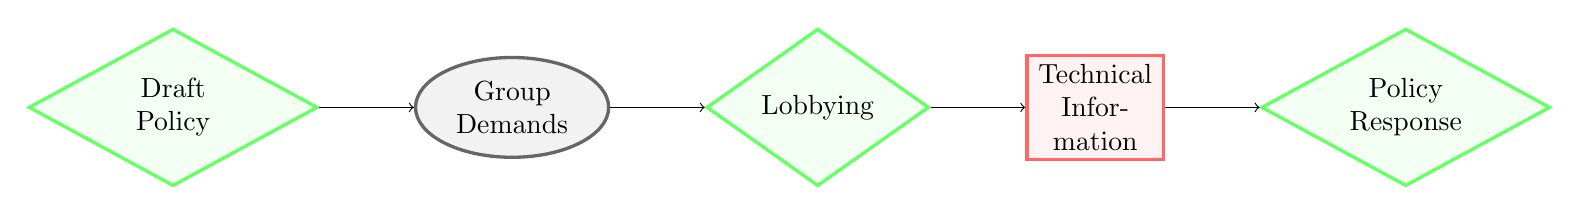
\begin{tikzpicture}[%
    node distance=1.2cm,
    auto,
    text width=1.5cm,
dnode/.style={diamond, align=center, aspect=2, fill=green!5,draw=green!60, very thick, minimum size=2cm},
squarednode/.style={rectangle, align=center, aspect=1, draw=red!60, fill=red!5, very thick, minimum size=1cm},
pnode/.style={ellipse, align=center, aspect=1, draw=black!60, fill=black!5, very thick, minimum size=1cm},
title/.style={rectangle, align=center, aspect=1, minimum size=2cm},
]
% Draft 
\node[dnode]      (draft)                     {Draft Policy};



% Group Nodes
\node[pnode]      (groupdemands) [right=of draft] {Group Demands};
\node[dnode]        (groupdecides) [right=of groupdemands] {Lobbying};
\node[squarednode]      (groupinfo) [right=of groupdecides] {Technical Information};

% policy 
\node[dnode]      (policy)       [right=of groupinfo] {Policy Response};
\draw[->] (groupinfo.east) -- (policy.west);
% \draw[->] (publicinfo.east) -- (policy.west);
% \draw[->] (principalinfo.east) -- (policy.south);
% \draw[->] (principalinfo2.east) -- (policy.south);

% Group Lines
\draw[->] (draft.east) -- (groupdemands.west);
\draw[->] (groupdemands.east) -- (groupdecides.west);
\draw[->] (groupdecides.east) -- (groupinfo.west);

% Titles
% \node[title]      (1) [above=of draft] {Policy};
%\node[title]      (2) [above=of groupdemands] {Preferences};
%\node[title]      (4) [above=of groupinfo] {Information/ Signal};
%\node[title]      (3) [above=of groupdecides] {Observed Behavior};


\end{tikzpicture}
\end{figure}
\normalsize


First, I offer a framework for assessing the causes of mass engagement. %In the remainder of this section, 
Next, I argue that organizations may mobilize large numbers of people for three reasons with observable implications for observed patterns of mass engagement and theoretical implications for predicted effects on policy. 


% better theory
\subsubsection{Incorporating political information into models of lobbying in rulemaking}
% MY THEORY 
% Representation 
% If all campaigns best fit the ``going down fighting'' type, then scholars are right to dismiss them. Below, I set these campaigns aside and elaborate on why mass mobilization may often be best understood as a tactic aimed at influencing policy.

% tactic
%Mass mobilization is a strategy. When successful, mass engagement is the result. 
An organization's ability to expand the scope of conflict by mobilizing a large number of people may occasionally be a valuable political resource. 
In contrast to scholars who focus on the deliberative potential of public comment processes, I focus on public engagement as a tactic aimed at gaining power.%, either by leveraging powerful ideas or engaging actors with the institutional power to shape decisions.
Scholars who do understand mobilization as a tactic \citep{Furlong1997, Kerwin2011} have thus far focused on organizations mobilizing their membership. %In contrast, 
I include a campaign's broader audience and its potential to grow, more akin to the concept of an attentive public \citep{Key1961} or issue public \citep{Converse1964}.

% public-private interests 
Appeals to the government are almost always couched in the language of public interest, even when true motivations are private \citep{Schattschneider1975}.
When lobbying during rulemaking, groups often make dubious claims to represent broad segments of the public \citep{Seifter2016UCLA}. %Mobilizing a large number of people may support such claims. 
If agency staff do not trust an organizations' representational claims, engaging actual people may be one of the few credible signals of a broad base of support. Furthermore, if organizations claim to represent people beyond their official members, reforms requiring groups to disclose information about their funding and membership \citep{Seifter2016UCLA} only go part way to assess groups' claims to represent these broader segments of the public. Indeed, if advocacy group decisions are primarily made by D.C. professionals, these advocates themselves may be unsure how broadly their claims resonate until potentially-attentive publics are actually engaged.

 Theorists may debate whether signing a petition of support without having a role in crafting the appeal is a meaningful voice or whether petitions effectively channel public interests, but, at a minimum, engaging a large number of supporters may help broader interests to distinguish themselves from truly narrower ones. It suggests that the organization is not ``memberless'' \citep{Skocpol2003} in the sense that they can demonstrate some verifiable public support.\footnote{
Public support can be faked or inflated using ``astroturf'' tactics but as I argue below, such campaigns ought to have observably different patterns of engagement.}


% resource - add David's cite 

% three insights 
Here I build on three insights. First, \citet{Furlong1997} and  \citet{Kerwin2011} identify mobilization as a tactic. The organizations that they surveyed reported that forming coalitions and mobilizing large numbers of people are among the most effective lobbying tactics. Second, \citet{Nelson2012} identify political information as a potentially influential result of lobbying by different business coalitions. While they focus on mobilizing experts, \citet{Nelson2012} describe a dynamic that can be extended to mass commenting: 
\begin{quote}
``strategic recruitment, we theorize, mobilizes new actors to participate in the policymaking process, bringing with them novel technical and political information. In other words, when an expanded strategy is employed, leaders activate individuals and organizations to participate in the policymaking process who, without the coordinating efforts of the leaders, would otherwise not lobby. This activation is important because it implies that coalition lobbying can generate new information and new actors---beyond simply the `usual suspects'---relevant to policy decision makers. Thus, we theorize consensus, coalition size, and composition matter to policy change.'' 
\end{quote}
I argue that, concerning political information, this logic extends to non-experts. The number and distribution of ordinary supporters may matter because it suggests a \textit{public} consensus. Instead of bolstering \textit{scientific} claims, a perceived public consensus bolsters \textit{political} claims.
Finally, \citet{Furlong1998}, \citet{Yackee2006JPART}, and others distinguish between direct and indirect forms of interest group influence in rulemaking. This distinction is especially important for political information, which may be most influential through indirect channels, such as through elected officials. In short, to understand how groups lobby in rulemaking, we must understand mass mobilization as a tactic aimed at producing political information that may have direct and indirect impacts on policymaking.% influence (see section \ref{influence-intro}). 


% PUBLIC OPINION and INFORMATION 
While most scholars have emphasized mass comments' lack of useful technical information, a few have raised their role in creating political information. \citet{Cuellar2005} calls on agencies to pay more attention to ordinary peoples' expressions of preference and \citet{Rauch2016} suggests that agencies reform the public comment process to include opinion polls. I build from a similar intuition that mass comment campaigns currently function like a poll or, more accurately, a petition, capturing the intensity of preferences among the attentive public---i.e., how many people are willing to take the time to engage.\footnote{
% public opinion example
For example, a campaign by the World Wildlife Federation provided language explicitly claiming to have public opinion on their side. Their model comment stated that ``Along with 80\% of the American people, I strongly support ending commercial trade in elephant ivory in the US.'' This suggests that mass comment campaigns aim to signal information about public opinion.
} 
Self-selection may not be ideal for representation, but opt-in participation---whether voting, attending a hearing, or writing a comment---may often be one of the few heuristics decisionmakers have about public preferences. 

Mobilizing citizens and generating new political information are key functions of interest groups in a democracy \citep{Mansbridge1992, Mahoney2007}. % The information generated by mass mobilization campaigns is explicitly political and more complex than an opinion poll. Activists aim to convince people which issues are important and how to think about them---mapping new issues and debates to familiar ones, thereby shifting the political landscape.  
Campaigns inform agencies about the distribution and intensity of opinions that are often too nuanced to estimate a priori. Many questions that arise in rulemaking lack analogous public opinion polling questions, making mass commenting a unique source of political information. 
As with public opinion on many specific policy issues,  most members of the public and their elected representatives may only learn about the issue and take a position as a result of a public pressure campaign \citep{Hutchings2003}. I thus consider public demands to be a latent factor in my model of policymaking (Figure \ref{fig:causal-whymail}). Public demands shape the decisions of groups who lobby in rulemaking. If they believe the attentive public is on their side, groups may attempt to reveal this political information to policymakers by launching a mass mobilization campaign. The public response to the campaign depends on the extent that the attentive public is passionate about the issue.%\footnote{It is difficult if not impossible to estimate public opinion, much less the intensity of such opinions before people have been made aware of the issue. Occasionally, increased awareness of a policy issue can radically alter its role in politics if a large number of people are given an opportunity to weigh in..."sleeping giants in Hutchings 2003?} 


\begin{figure}[h!]
    \centering
    \caption{Incorporating Mass Engagement and Political Information into Models of Lobbying}
    \label{fig:causal-whymail}
\tiny
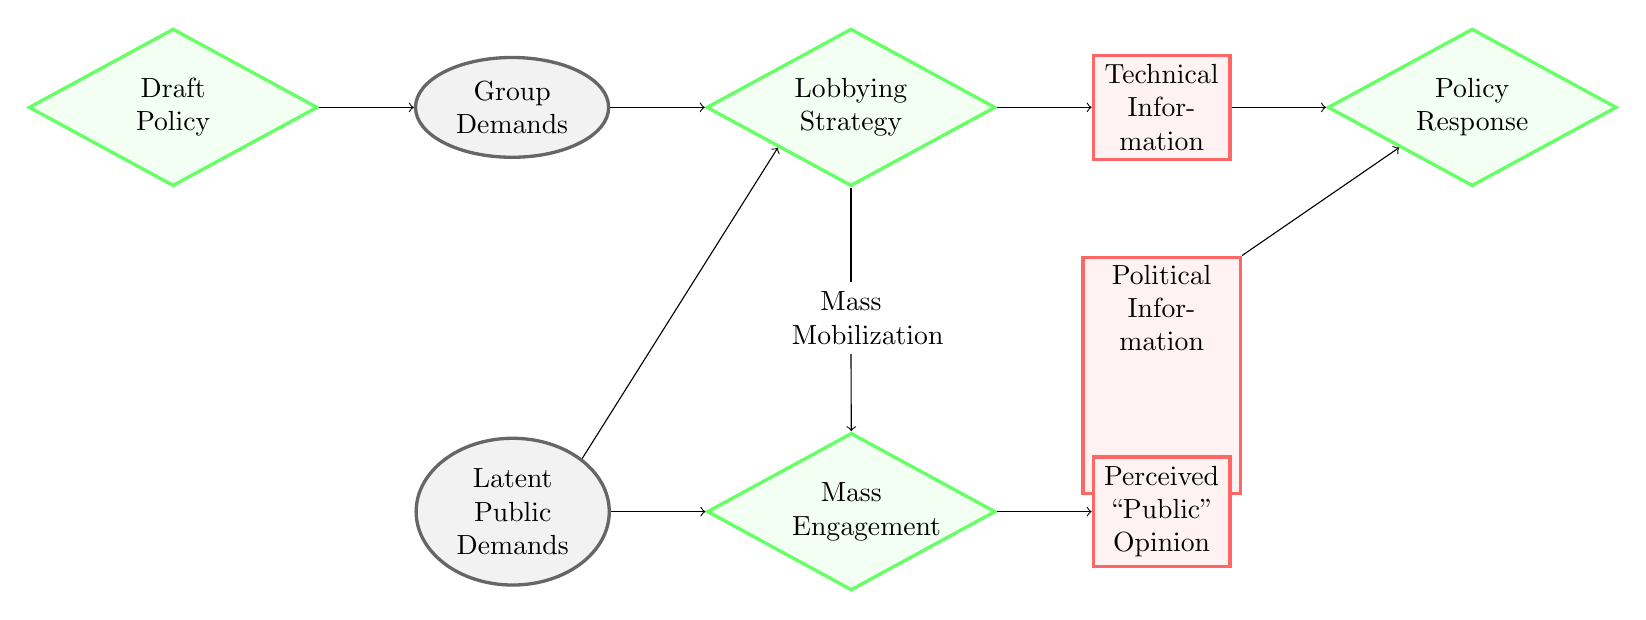
\begin{tikzpicture}[%
    node distance=1.2cm,
    auto,
    text width=1.5cm,
dnode/.style={diamond, align=center, aspect=2, fill=green!5,draw=green!60, very thick, minimum size=2cm},
squarednode/.style={rectangle, align=center, aspect=1, draw=red!60, fill=red!5, very thick, minimum size=1cm},
pnode/.style={ellipse, align=center, aspect=1, draw=black!60, fill=black!5, very thick, minimum size=1cm},
title/.style={rectangle, align=center, aspect=1, minimum size=2cm},
]
% Draft 
\node[dnode]      (draft)                     {Draft Policy};



% Group Nodes
\node[pnode]      (groupdemands) [right=of draft] {Group Demands};
\node[dnode]        (groupdecides) [right=of groupdemands] {Lobbying Strategy};
\node[squarednode]      (groupinfo) [right=of groupdecides] {Technical Information};

% policy 
\node[dnode]      (policy)       [right=of groupinfo] {Policy Response};
\draw[->] (groupinfo.east) -- (policy.west);
% \draw[->] (publicinfo.east) -- (policy.west);
% \draw[->] (principalinfo.east) -- (policy.south);
% \draw[->] (principalinfo2.east) -- (policy.south);

% Group Lines
\draw[->] (draft.east) -- (groupdemands.west);
\draw[->] (groupdemands.east) -- (groupdecides.west);
\draw[->] (groupdecides.east) -- (groupinfo.west);

% Titles
% \node[title]      (1) [above=of draft] {Policy};
% \node[title]      (2) [above=of groupdemands] {Preferences};
% \node[title]      (4) [above=of groupinfo] {Information/ Signal};
% \node[title]      (3) [above=of groupdecides] {Observed Behavior};
% \node[title]      (5) [above=of policy] {Policy'};

% political info
\node[rectangle, minimum width =2cm, minimum height = 3cm, draw=red!60, fill=red!5, very thick]      (politicalinfo) [below=of groupinfo] {};
\node[text centered]      (politicalinfotext) [below=of groupinfo] {Political Information};
\node[text centered]      (mobilizing) [below=of groupdecides] {Mass\\ Mobilization};
\draw[->] (politicalinfo.north east) -- (policy.south west);

% public Nodes
\node[squarednode]      (publicinfo) [below=of politicalinfotext] {Perceived ``Public'' Opinion};
\node[dnode]      (publicdecides) [left=of publicinfo] {Mass\\ Engagement};
\node[pnode]        (publicdemands) [left=of publicdecides] {Latent Public Demands};

% public Lines
% \draw[->] (draft.east) -- (publicdemands.west);
\draw[->] (publicdemands.east) -- (publicdecides.west);
\draw[->] (publicdemands.north east) -- (groupdecides.south west);
\draw[-] (groupdecides.south) -- (mobilizing.north);
\draw[->] (mobilizing.south) -- (publicdecides.north);
\draw[->] (publicdecides.east) -- (publicinfo.west);



\end{tikzpicture}
\end{figure}
\normalsize

Figure \ref{fig:causal-whymail} amends the Classic Model of interest group lobbying (Figure \ref{fig:causal-classic-lobbying}) to incorporate the above intuitions. In addition to providing technical information, for example through sophisticated comments, an organization may mobilize supporters. The more support a group has, the more successful this effort will be. Large-scale engagement may produce several types of relevant political information. The most direct and obvious is the expressed ``public opinion'' that policymakers observe.\footnote{I address other types of political information that mass engagement may create elsewhere. For an expanded model, see Figure \ref{fig:causal-full} in the Appendix.}

The causal process visualized in Figure \ref{fig:causal-whymail} only operates under certain conditions, one of those being that mobilization is aimed at influencing policy. 
% As I will describe in section \ref{influence-intro}, another condition is that agencies have the capacity to process political information. 
%But first, section \ref{principals-intro} focuses on another key source of political information: political oversight behavior.
% Another condition is that the ...This latter condition is key to the present question of why mass engagement occurs.
% In order to answer this question, we need a theory why mass commenting occurs and systematic analysis of public commenting behavior in agency rulemaking. 




\subsubsection{Hypotheses about the drivers of mass mobilization}

% TYPES OF CAMPAIGNS AND COALITIONS
\subsubsection{Types of campaigns} The outcomes of mass mobilization depend, in part, on the aims of a campaign. I distinguish group campaigns by which of three distinct aims they pursue: (1) to win concessions by going public, (2) to disrupt a perceived consensus, or (3) to go down fighting. Going public and disrupting a perceived consensus are forms of proactive and reactive outside lobbying, respectively. Here, going down fighting describes any situation where the organization does not expect to influence policy but mobilizes for other reasons. 

\textbf{Going public.} Coalitions ``go public'' when they believe that expanding the scope of conflict gives them an advantage.\footnote{
``Going public,'' ``outside lobbying'' or an ``outside strategy'' contrasts with insider lobbying. It is used by Presidents \citep{Kernell2007}, Members of Congress \citep{Malecha2012}, interest groups \citep{Walker1991, Dur2013}, Lawyers, and Judges (Davis 2011). 
For example, organizations may use phone banks, targeting strategies, and direct-mail techniques to drum-up and channel public support (Cooper 1985).
}
As these are the coalitions that believe they have more intense public support\footnote{
This strategy is likely to be used by those disadvantaged (those \citet{Schattschneider1975} calls the `losers') in a policy process with less public attention.
%Rulemaking with little public attention is the norm, and nearly all scholarship on rulemaking in political science thus focuses on interest-group and inter-branch bargaining, rather than public opinion and social movements.
}, mass engagement is likely to skew heavily toward this side. Indeed, \citet{Potter2017} finds that advocacy group-driven campaigns mobilize far more people on average than industry-driven campaigns. Additionally, many people may be inspired indirectly (e.g., through news stories) or to engage with more effort (e.g., writing longer comments) than people mobilized by the side with less public support.  This is important because political information may be especially influential if decisionmakers perceive a consensus.\footnote{
For example, consensus among interest groups \citep{Golden1998, Yackee2006JPART}, especially business unity \citep{Yackee2006JOP, Haeder2015}, predicts policy change, though it is not clear if this is a result of strategic calculation, a perceived obligation due to the normative power of consensus (e.g., following a majoritarian logic \citep{Mendelson2011}), or simply that unified demands are easier to process than opposing demands.
}

\begin{subhyp}

\begin{hyp} \label{hyp:support}
Lobbying coalitions mobilize mass engagement when they perceive the attentive public is on their side, have sufficient resources, and perceive an opportunity to influence policy.
\end{hyp}

The key part of this hypothesis is that mobilizing is correlated with existing public support, what might be called ``grass-roots'' support. The converse, that organizations mobilize when they have less public support, could also be true. For example, business groups who are already advantaged in low salience rulemaking may decide to leverage their superior resources further to mobilize support to alter a bad reputation or bolster claims that they represent more than their private interest. If mobilization most often takes this ``astro-turf'' form, this would be evidence against Hypothesis \ref{hyp:support} and Schattschneider's argument that it is the disadvantaged who seek to expand the scope of the conflict. 

The latter parts of Hypothesis \ref{hyp:support} regarding sufficient resources and political opportunity are scope conditions. Most organizations that are disadvantaged in low-salience rulemaking also lack resources to launch mass mobilization campaigns. If an organization does not perceive a lobbying opportunity, it would be incorrect to call mobilization a lobbying strategy. Many factors may contribute to perceived political opportunities. For example, \citet{Moore2017} finds that agencies that use high levels of expertise (as defined by \citet{Selin2015}) receive fewer comments, possibly because mobilizing organizations perceive these rules to be less open to influence. 

\textbf{Disrupting a perceived consensus.} I theorize that when coalitions with less public support mobilize, it is a reaction to their opponents. Because the impression of consensus is powerful, when a coalition goes public, an opposing coalition may countermobilize. Because I theorize that these are coalitions with less intense public support and its aim is prevent a perceived consensus, I expect such campaigns to engage fewer people, less effort per person, and yield a smaller portion of indirect engagement. 


\begin{hyp} \label{hyp:disrupt}
When a lobbying coalition with more intense public support mobilizes successfully in response to an opportunity to influence policy, opposing coalitions with less public support are more likely to counter-mobilize, but with proportionally smaller results.
\end{hyp}

The first part of Hypothesis \ref{hyp:disrupt} would be undermined if lobbying organizations with less public support are no more likely to engage in outside lobbying when their opposition does so. While \citet{Potter2017} found industry groups were no more likely to advocate for rules to be strengthened, weakened or withdrawn, this does not mean that they are no more likely to mobilize when their opposition does so.

The second part of this hypothesis, that countermobilization is proportionally smaller, rests on the intuition that the scale and intensity of public engagement are moderated by preexisting support for the proposition that people are being asked to support. It is possible that the ``potentially mobilized'' segments of the public are unrelated to public support before being contacted by the campaign, for example, if mobilization is driven more by partisan identities than issue preferences.

\textbf{Going down fighting.} Finally, campaigns may target supporters rather than policymakers. Sometimes organizations ``go down fighting'' to fulfill supporters' expectations.
I use ``going down fighting'' as shorthand for campaigns aimed only at fulfilling member, donor, or supporter expectations and related logics that are internal to the organization, including member retention or recruitment, fundraising, or satisfying a board of directors. For example, as Figure \ref{fig:sierra} shows, the Sierra Club uses campaigns to collect contact information of supporters and potential members. In this case, given the executive-branch transition between 2010 when the rule was initiated and 2017 when it was delayed, the Sierra Club may have had little hope of protecting methane pollution standards, but for members of the public who wanted to voice their opinion, the Sierra Club created an easy way to do so, as long as users consented to ``receive periodic communication from the Sierra Club.'' 

\begin{figure}
    \caption{Mass mobilization campaign by the Sierra Club collects contact information}
    \centering
    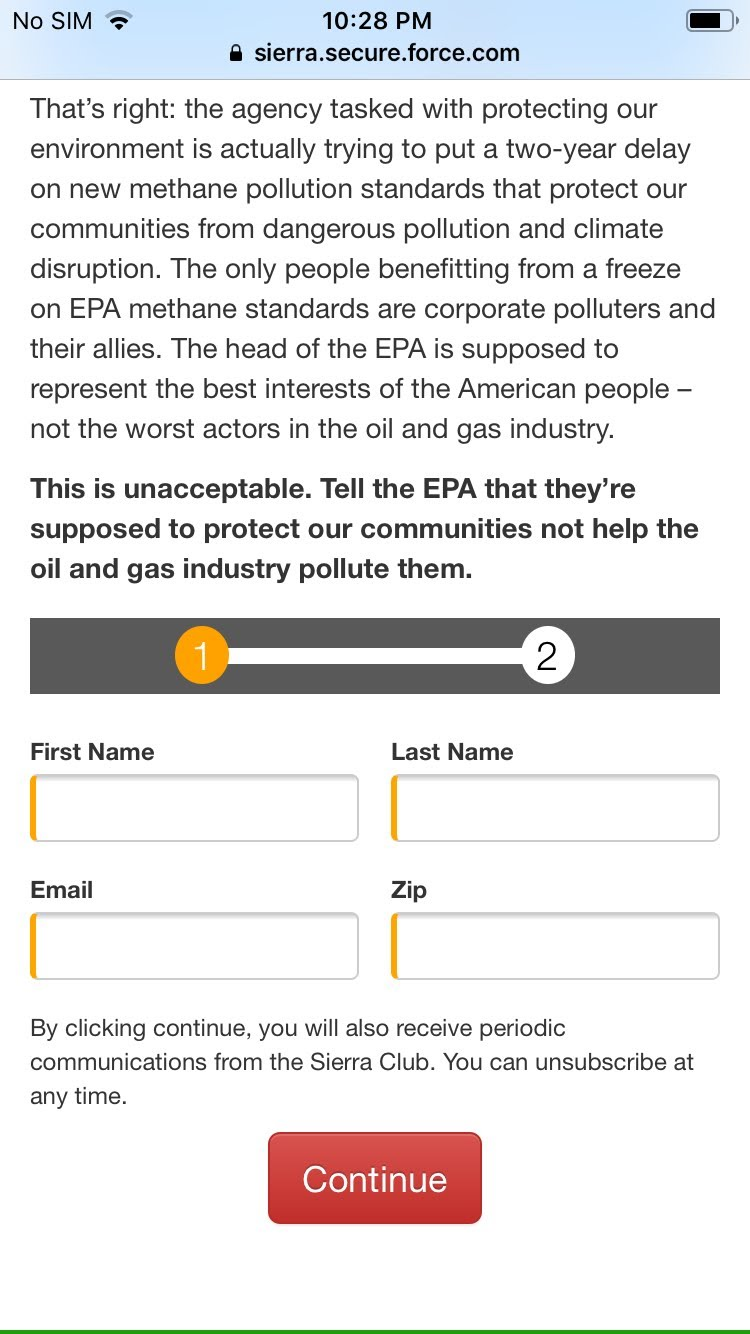
\includegraphics[height = 4in]{Figs/sierra1.jpeg}
    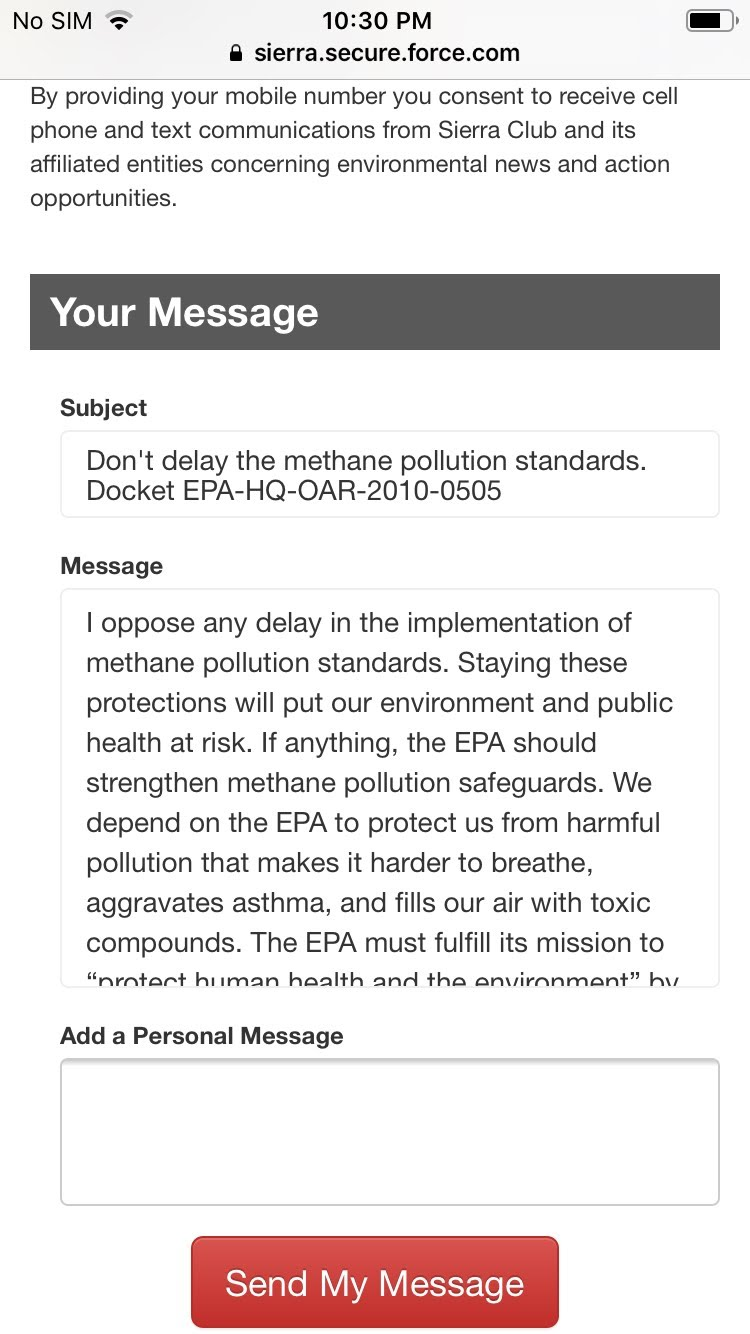
\includegraphics[height = 4in]{Figs/sierra2.jpeg}
    \label{fig:sierra}
\end{figure}

While such campaigns may engage many people, they are unlikely to affect policy or to inspire countermobilization. I expect such campaigns to occur on rules that have high partisan salience (e.g., rules following major legislation passed on a narrow vote), rules that propose large shifts on policy issues dear to member-funded public interest groups, or rulemaking started shortly after presidential transitions when executive-branch agendas shift more quickly than public opinion.

\begin{hyp}
When a lobbying coalition with more intense public support successfully mobilizes for reasons other than influencing policy, opposing coalitions with less public support are not more likely to counter-mobilize.
\end{hyp}

Going public and going down fighting may be difficult to distinguish in the observed public response. Indeed, members of the public may poorly understand the different chances of success in each case. However, lobbying organization do likely know their chances of success and should thus invest less in sophisticated insider lobbying under the going down fighting strategy. By identify cases where coalitions engage in large public campaigns without corresponding investment in sophisticated lobbying, I can assess whether countermobilization and is indeed less likely in these cases. Table \ref{tab:campaigns-patterns} specifies the general pattern of engagement suggested by each of the three reasons behind mass-comment campaigns. 

% CAMPAIGNS-PATTERNS TABLE 
\begin{table}
\small
\centering 
  \caption{Observable differences in engagement across types of mass-mobilization campaigns}
  \def\arraystretch{1.5}
\begin{tabular}{@{\extracolsep{5pt}} lcccc} 
& Inside &  & Outside &   \\ \cline{3-5} 
& Technical information & Number of comments & Effort & Contagion \\
\hline
Going public & High & High & High & High  \\ 
\hline
Disrupting  & High & Low & Low & Low  \\
\hline
Going down fighting & Low & High & High & High  \\ 
\hline 
\end{tabular}
\label{tab:campaigns-patterns}
\end{table}


As Table \ref{tab:campaigns-patterns} suggests, the relevant statistic distinguishing patterns is the \textit{relative} number of each type of comment on each side on a given rulemaking docket. Even among rules targeted by campaigns, salience varies significantly and thus ``high'' and ``low'' numbers of comments will differ across rules. Importantly, even campaigns that achieve very low public response rates appear in these data. Because campaigns aim to collect thousands of comments, it is implausible that even the most unpopular position would achieve no supportive responses. For example, \citet{Potter2017} found Poultry Producers averaging only 319 comments per campaign. While this is far from the Sierra Club's average of 17,325 comments per campaign, it is also far from zero.

% \subsection{Mobilizing for Recruitment}
% A third possibility is that mobilization around bureaucratic decisions is unrelated to the possibility of affecting policy and primarily a way to recruit and engage members or raise the profile of the movement. If this is the case, behaviors like protesting and mass commenting on rules are largely epiphenomena to unrelated kinds of politics. Organizers may know that mobilization has minimal effects, but lead members to engage as a means to other ends. Many of the mobilized themselves may doubt their efficacy but still take advantage of the opportunity to protest. 

\paragraph{Public and private goods.} While coalitions may form around various material and ideological conflicts, those most likely to be advantaged by going public or going down fighting are public interest groups---organizations primarily serving an idea of the public good rather than the material interests of their members.\footnote{\citet{Potter2017} similarly distinguishes ``advocacy groups'' from ``industry groups.'' \citet{Berry1999} calls these groups ``citizen groups'' and emphasizes conflict over cultural issues. While some public interest groups focus on conservative or progressive cultural issues, like religious education, immigration, or endangered species, many are more focused on the public provision or protection of public goods such as national parks, consumer product safety standards, air quality, drinking water, and public safety.

One exception may be types of membership organizations that are both broad and often focused on material outcomes for their members such as labor unions. \citet{Potter2017} puts unions in the ``Industry'' category. I take a different approach based on the coalition with whom such groups lobby. If a union lobbies alongside businesses, I classify this as a private interest-driven coalition. If a union lobbies with public interest groups on public health or safety issues, I classify this as a public interest.} Thus, I theorize that mass mobilization is most likely to occur in conflicts of public versus private interests or public versus public interests (i.e., between coalitions led by groups with distinct cultural ideals or desired public goods), provided they have sufficient resources to run a campaign.
If true, one implication is that mass mobilization will systematically run counter to concentrated business interests where they conflict with the values of public interest groups with sufficient resources to mobilize.


\begin{hyp} \label{hyp:publicinterest}
Public interest group coalitions mobilize more often than business-driven coalitions.
\end{hyp}

Hypothesis \ref{hyp:publicinterest} posits a conditional logic in the decision to mobilize. If resources purely determined outside lobbying, business-driven coalitions would often dominate, as they do elsewhere. However, I argue, because outside lobbying can alter the decision environment, those who have the advantage in the usual rulemaking process (where a more limited set of actors participate) have little incentive to expand the scope of the conflict.




% We do not know who engages in mass commenting. Some assume that people who engage in mass commenting belong to membership organizations. Others imply that they are people who happen to have an opinion. RAUCH discusses both "members" and  _______
% % The people who engage in mass commenting are often assumed to be 

% Engaging a broader audience and thus changing the scope of conflict is a basic political strategy. Presidents, supreme court justices, and others "go public" when doing so alters their opponents' calculations. 

% Which campaigns engage a broader audience and which do not? 


\subsubsection{Types of public engagement} I classify supporters into three types that help describe key pieces of political information. I illustrate these types in the context of public comments. Comments that are exact copies of a form letter are akin to petition signatures from supporters who were engaged by a campaign to comment with minimal effort. Commenters that also take time to add text indicate more intense preferences. Finally, commenters who express solidarity in similar but distinct phrases indicate they were engaged indirectly, perhaps by a news story or a social media post about the campaign, as campaign messages spread beyond those initially targeted.\footnote{It is possible that some people in this latter category engage purely on their own initiative, but any impact they have likely comes from their alignment with a coalition. Furthermore, as I show below, wholly original comments are rare.} Because the success of a mobilization effort is moderated by public support, broader public interest group coalitions ought to mobilize more people, more effort per person, and more people indirectly for the same amount of mobilization effort (e.g., spending or solicitations).  

\begin{hyp}
Public interest group coalitions mobilize more successfully than business-driven coalitions. Indicators of success include (1) the number of comments supporting a coalition (2) the effort per comment (3) the number of comments mobilized indirectly. 
\end{hyp}

\end{subhyp}

The size of each group thus offers political information to policymakers, including coalition resources, the intensity of sentiment, and the potential for conflict to spread. The first two types signal two kinds of intensity or resolve. First, they show the mobilizers' willingness to commit resources to the issue. Second, costly actions show the intensity of opinions among the mobilized segment of the public \citep{Dunleavy1991}. The number of people engaged by a campaign is not strictly proportional to an organization's investment. The less people care, the more it costs to mobilize them. The third type indicates potential contagion. Indications that messages spread beyond those initially targeted may be especially powerful \citep{Kollman1998}. 

Information about organizational resolve, the intensity of public demands, and contagiousness are thus produced, but %, as discussed in section \ref{influence-intro},
such political information will only influence decisions if these signals are processed in a way that captures this information and relays it to decisionmakers. These organizational processes may vary significantly across agencies.





%%%%%%%%%%%%%%%%%%%%%%%%%%%%%%%%%%%%%%%%%%%%%%%%%%%%%%%%%%%%
\section{Methods}

\subsection{Measuring mass engagement and political information}
\label{whyMail-methods}
In this section, I develop methods to attribute mass comments to the campaigns that mobilized them and measure the intensity of preferences expressed. 
To link individual comments to the more sophisticated lobbying efforts they support, I use text reuse and topic models to identify clusters of similar comments, reflecting formal and informal coalitions. Comments with identical text indicate which groups and coalitions also chose to run a mass comment campaign. Within each campaign, I measure the intensity and potential for the movement to grow. To measure intensity, I examine the ratio of high-effort and low-effort comments. To measure potential to grow, I measure the number of comments mobilized indirectly by the campaign.
The result is several new measures that paint a picture of mass commenting. Using these new measures of public engagement in agency rulemaking, I identify the conditions under which it occurs and produces different politically-relevant information. 

\subsubsection{Who lobbies?}
Previous studies of rulemaking stress the importance of coalitions \citep{Yackee2006a}. Scholars have measured coalitions of organized groups but have yet to be able to attribute citizen comments to the coalition that mobilized them.
% Metadata on participants in rulemaking including the date and author of comments (often including the type of author, i.e. business, business group, citizen, public interest group, etc.)% and briefs
% allows me to track and compare relative alignment across venues and over time to assess whose ideas and interests are reflected at each stage of policymaking and in policy processes over time. % and review, for example from a statute or executive order, to the agency rule(s), to review by the White House, to court opinions. 
Unfortunately, metadata on the authors of comments are often inconsistent and incomplete. As this information is key to identifying influential actors, improving these data is a significant data-organization task. I have collected a corpus of over 70 million comments on over 300,000 proposed rules. The first task will be linking these comments to other data on the rules. 

Text search matching organization and individual names across texts, especially those named as comment authors will help systematically link individuals to the groups that mobilized them.% who may participate in different coalitions and under different names over time. 
This helps to identify formal coalitions of organizations that sign onto the same comment as well as experts and citizens mobilized by advocacy campaigns to submit separate comments.

Having identified who is participating in rulemaking, the next step is to identify who is lobbying together.

\subsubsection{Who lobbies together?}
% political information example 
The Oceana coalition framed its mass mobilization effort to curb the  Bureau of Ocean Energy Management's 2017 Proposed Offshore Oil and Gas Leasing Program as a ``petition signed by 67,275 self-proclaimed United States residents,'' suggesting that organizations consider these efforts as akin to petitions. In the same statement, Oceana also claimed the support of ``more than 110 East Coast municipalities, 100 Members of Congress, 750 state and local elected officials, and 1,100 business interests, all of whom oppose offshore drilling,'' suggesting that claims of public and elected official support aim to provide similar kinds of political information. 

% lobbying together - cosigning 
When actors sign onto the same comment, it is clear that they are lobbying together. This generally takes two forms. Businesses and groups representing allied industries often co-sign carefully crafted suggestions that reflect their common interest. We expect this to occur when the benefits of coordination outweigh the costs \citep{Yackee2006JOP}. The other form this take is public campaigns that ask citizens to submit a form letter, often alongside other actions such as protests. These occasional bursts of civic participation may affect rulemaking \citep{Coglianese2001}, but this is yet to be tested. In the first form, many of the businesses are repeat players and I record them individually. In the second form, the advocacy groups are repeat players, and I recorded their participation, but it would be citizens who participate are likely not and I record the number of these comments as an amplitude parameter for the text they signed and I attribute form-letter texts to the advocacy groups promoting them.

Various businesses, advocacy groups, and citizens often comment separately even when they aligned. The comment process is open to anyone and it is often not worthwhile for all actors to coordinate their messages. There may be many dimensions of demands and it is unclear to which coalition many comments belong.

% Identifying when commenters change coalitions is key for testing policy feedback theories about how policies reorganize political coalitions. I do this by indexing rules over time and adding a parameter for the probability that an actor switches from one coalition to another at each point in time. This allows the model to achieve a better fit by reclassifying an actor after some point in time. These actor-specific and coalition-specific points in time are a key output of this approach required to test theories of how policies reorganize political coalitions. 

% Bounding the scope of this model (i.e. the policy system) is a challenge. On the one hand, each agency deals with many issues of interest to different coalitions. On the other hand, many lobby across multiple agencies. I opt to model coalition advocacy at a fine scale based on Office of Management and Budget agency sub-function codes, but I may try to link across related issues and agencies. 

In addition to mapping text re-use, I adapt several statistical models (Bayesian classifiers) of text to classify comments into coalitions. Classifying comments into common groups is a task well suited for a single membership topic model.\footnote{
This is in contrast to the mixture model I use to estimate the distribution of multiple topics in each document and each coalition in section \ref{principals-methods}
}. 
This model clusters documents by the frequency with which they use different words. Being classified together does not mean that the documents all address exactly the same distribution of substantive issues, just that how issues are discussed is similar relative to the full set of documents.
I start by modeling all comments on each rule (collapsing exactly identical comments to one document) with three topics, which I will then inspect to see how well the comments of named organizations were classified. If three topics appear to sensibly describe the conflict, I tag these topics as ``pro, con, other.'' 





In terms of the causal process theorized above, this section focuses on measuring and explaining organizations' lobbying choices (i.e. to only provide technical information or to also mobilize) and public response to mobilization campaigns (the frequency and effort with which people engage). The key explanatory variable is public support for the campaign. The bold arrows in figure \ref{fig:causal-whymail-test} indicate the relationships of interest for this step.

\begin{figure}[h!]
    \centering
    \caption{Step 1: Explaining Mass Mobilization and Mass Engagement} 
    \label{fig:causal-whymail-test}
\tiny
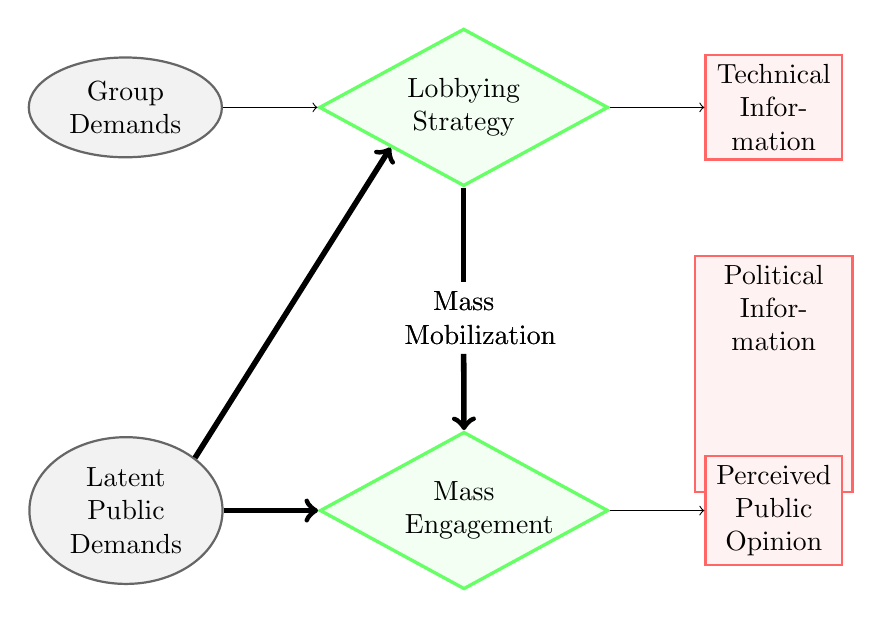
\begin{tikzpicture}[%
    node distance=1.2cm,
    auto,
    text width=1.5cm,
dnode/.style={diamond, align=center, aspect=2, fill=green!5,draw=green!60, very thick, minimum size=2cm},
squarednode/.style={rectangle, align=center, aspect=1, draw=red!60, fill=red!5, thick, minimum size=1cm},
pnode/.style={ellipse, align=center, aspect=1, draw=black!60, fill=black!5, thick, minimum size=1cm},
title/.style={rectangle, align=center, aspect=1, minimum size=2cm},
]

% Group Nodes
\node[pnode]      (groupdemands) {Group Demands};
\node[dnode]        (groupdecides) [right=of groupdemands] {Lobbying Strategy};
\node[squarednode]      (groupinfo) [right=of groupdecides] {Technical Information};


% Group Lines
\draw[->] (groupdemands.east) -- (groupdecides.west);
\draw[->] (groupdecides.east) -- (groupinfo.west);

% Titles
% \node[title]      (1) [above=of draft] {Policy};
% \node[title]      (2) [above=of groupdemands] {Preferences};
% \node[title]      (4) [above=of groupinfo] {Information/ Signal};
% \node[title]      (3) [above=of groupdecides] {Observed Behavior};
% \node[title]      (5) [above=of policy] {Policy'};

\node[text centered]      (mobilizing) [below=of groupdecides] {Mass\\ Mobilization};

% political info
\node[rectangle, minimum width =2cm, minimum height = 3cm, draw=red!60, fill=red!5,  thick]      (politicalinfo) [below=of groupinfo] {};

\node[text centered]      (politicalinfotext) [below=of groupinfo] {Political Information};

\node[text centered]      (mobilizing) [below=of groupdecides] {Mass\\ Mobilization};

\node[squarednode]      (publicinfo) [below=of politicalinfotext] {Perceived Public Opinion};
\node[dnode]      (publicdecides) [left=of publicinfo] {Mass\\ Engagement};
\node[pnode]        (publicdemands) [left=of publicdecides] {Latent Public Demands};


% public Lines
\draw[->, line width=2] (publicdemands.east) -- (publicdecides.west);
\draw[->, line width=2] (publicdemands.north east) -- (groupdecides.south west);
\draw[-, line width=2] (groupdecides.south) -- (mobilizing.north);
\draw[->, line width=2] (mobilizing.south) -- (publicdecides.north);
\draw[->] (publicdecides.east) -- (publicinfo.west);



\end{tikzpicture}
\end{figure}
\normalsize

% OUTCOMES OF A CAMPAIGN




\subsubsection{Measuring the volume, intensity, and potential contagion of public engagement.}

%\textbf{Level of engagement.} 
% Dependent variables include the number of people engaged and the effort per comment.
I argue that activists' opportunities and strategies explain variation in engagement, which I measure in several ways. 

\paragraph{Volume.} 
First, I measure the total number of comments on the rule. As commenting are the results of two processes: deciding to lobby at all and then deciding to mobilize, the distribution contains many cases where groups may have had success mobilizing but never reached the choice of whether to mobilize or not. Perhaps they were unaware of the draft rule. Once the decision to mobilize has been reached and made, the result of mobilizing is a count process. Thus, the count of comments fits a zero-inflated negative binomial distribution. When focusing on coalitions, we have already subset to cases where mobilization occurred and thus commenting can now be considered a regular count process. 

\textbf{Effort.} Effort per comment is a continuous measure of the of the number of words people write, omitting any to text longer than 10 words provided by a mobilizing organization. % effort example 
For example, using the form shown in \ref{fig:sierra}, the Sierra Club mobilized more than 47,710 people to submit exactly the same text on the delay of the methane pollution rule, but 7,452 people also took the time to write a personalized comment in addition to the form letter text. However, we may not observe people who have low levels of passion for the issue because they either do not cross the effort threshold required to comment or opt to write nothing more than the form letter. Thus the low end of the distribution of words is truncated.

% contagion
\textbf{Contagion.} Mass-comment campaigns have wildly different results. Some gather a clean 10,000 copies of (or, more accurately, signatures on) the same comment and call their work done. Others ``go viral''---inspiring a mess of further engagement where the original messages are translated through social media posts and news stories.
%Within each coalition, I look for text re-use, identifying strings longer than 10 words that are repeated to identify the share of unique comments that likely resulted from direct mobilization versus indirect engagement. 
Finally, I count the number of people who use fewer than 10 words matching an organizational comment, plausibly those who were mobilized indirectly, another regular count process.

\begin{quote}
\textbf{Dependent Variables:} 

Model 1) Total comments $\sim$ zero-inflated negative binomial; 

Model 2) Comments per coalition $\sim$ negative binomial; 

Model 3) Effort per comment $\sim$ truncated normal; 

Model 4) Contagion $\sim$ negative binomial. 

% Model 4) Type of campaign $\sim$ multinomial. 
\end{quote}

The dependent 2-4 are built using text reuse and bayesian classifiers\footnote{
Ultimately something similar to the correlated topic model \citep{Blei2005}, possibly with lexical priors \citep{Fong2016} based on organizational comments
},
one observation per coalition per rule. Explanatory variables include agency alignment with Congress and the president (models 1-4), coalition unity and alignment (models 2-4), and coding coalitions as driven more by public or private interests (models 2-3).%, part of the DV in model 4).





%Political scientists have thus far focused on sophisticated lobbying efforts. However, as 
\paragraph{Data.}
In his case-study of several rules, \citet{Cuellar2005} finds that ``contrary to conventional wisdom, comments from the lay public make up the vast majority of total comments about some regulations. This shows at least some potential demand among the mass public for a seat at the table in the regulatory process.'' 
Having collected over 70 million comments on over 300,000 proposed rules, I am able to offer a much more systematic analysis. Figure \ref{fig:comments-mass} shows all comments posted on regulations.gov over time by whether they are exact copies of another comment or not. This highly restrictive definition of what counts as mass engagement captures comments that were certainly mobilized by a campaign. As \ref{fig:comments-mass} shows, not only are most comments are from ordinary people, but the vast majority of comments are mobilized by mass commenting campaigns.

\begin{figure}[h!]
    \centering
        \caption{Unique vs Form-letter Comments Posted to Regulations.gov 2006-2018}
    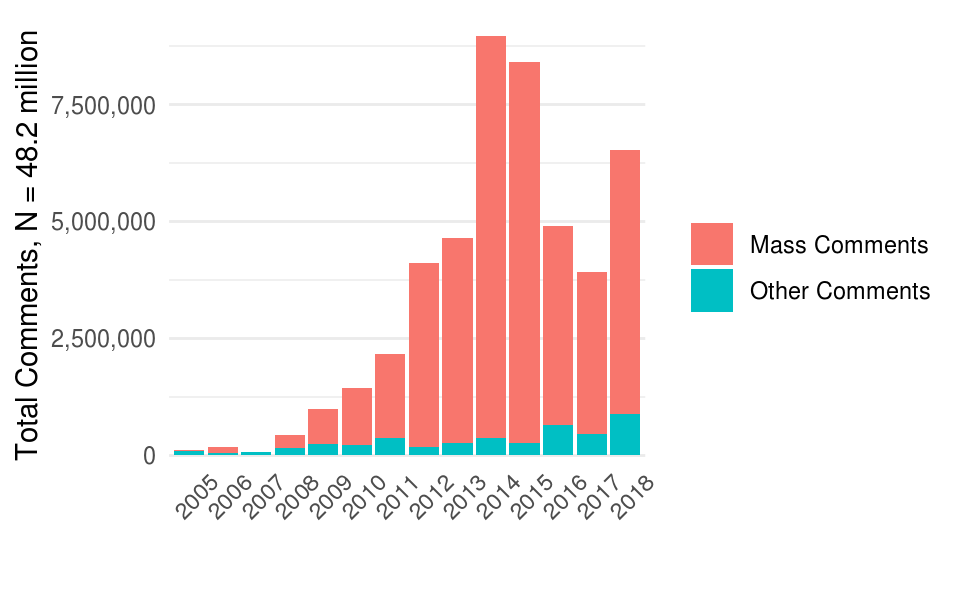
\includegraphics[height =2in]{Figs/comments-mass-vs-unique-1.png}
    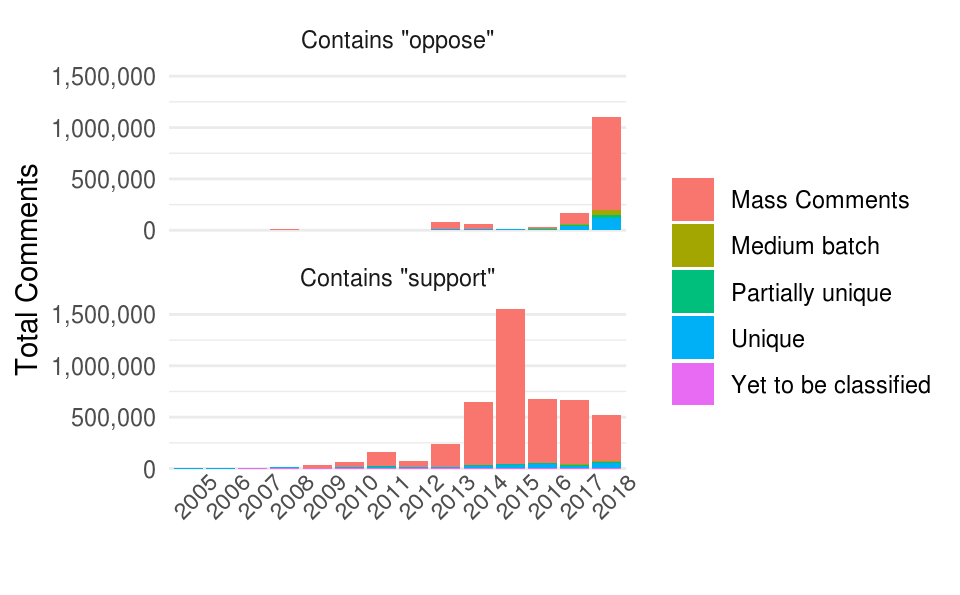
\includegraphics[height =2in]{Figs/comments-mass-support-vs-oppose-1.png}

    \label{fig:comments-mass}
\end{figure}

The right pane of \ref{fig:comments-mass} shows results from a sample of several million comments for which I have digitized the texts. Many of these comments are in support proposed agency rules, as was the case with both the do not call and mercury rule examples. A rough measure of support (whether the comment text includes the word `` support '' or `` oppose '') shows that many more comments mention support, until 2018, when there is a fairly dramatic reversal in the share of comments mentioning `` support '' compared to those mentioning ` `oppose '' (figure \ref{fig:comments-mass}). 







%%%%%%%%%%%%%%%%%%%%%%%%%%%%%%%%%%%%%%%%%%%%%%%%%%%%%%%%%%%%
% RESULTS
\section{Patterns of public engagement in rulemaking}
\label{whyMail-results}

%In this section, I present the results of applying the classification methods described above.

\paragraph{Most comments result from mass-comment campaigns.}
Figure \ref{fig:comments-support} shows all comments posted on regulations.gov over time by whether they are exact or partial copies of another comment or not. While some agencies classify all duplicate comments as mass comments, I call comments that have between 2 and 99 identical copies, ``medium batch'' because such comments may reflect coordinated efforts among interest groups that do not include a public pressure strategy that involves mobilizing ordinary people. Here ``mass comments'' are comments that have either 100 or more identical copies or were uploaded in bulk batches of at least 100. This restrictive definition of what counts as mass engagement captures comments that were certainly mobilized by a campaign. As Figure \ref{fig:comments-support} shows mass commenting campaigns mobilize the vast majority of comments. In other words, most comments are from ordinary people.

\begin{figure}[h!]
    \centering
        \caption{Comments on Draft Rules Posted to Regulations.gov 2006-2018}
    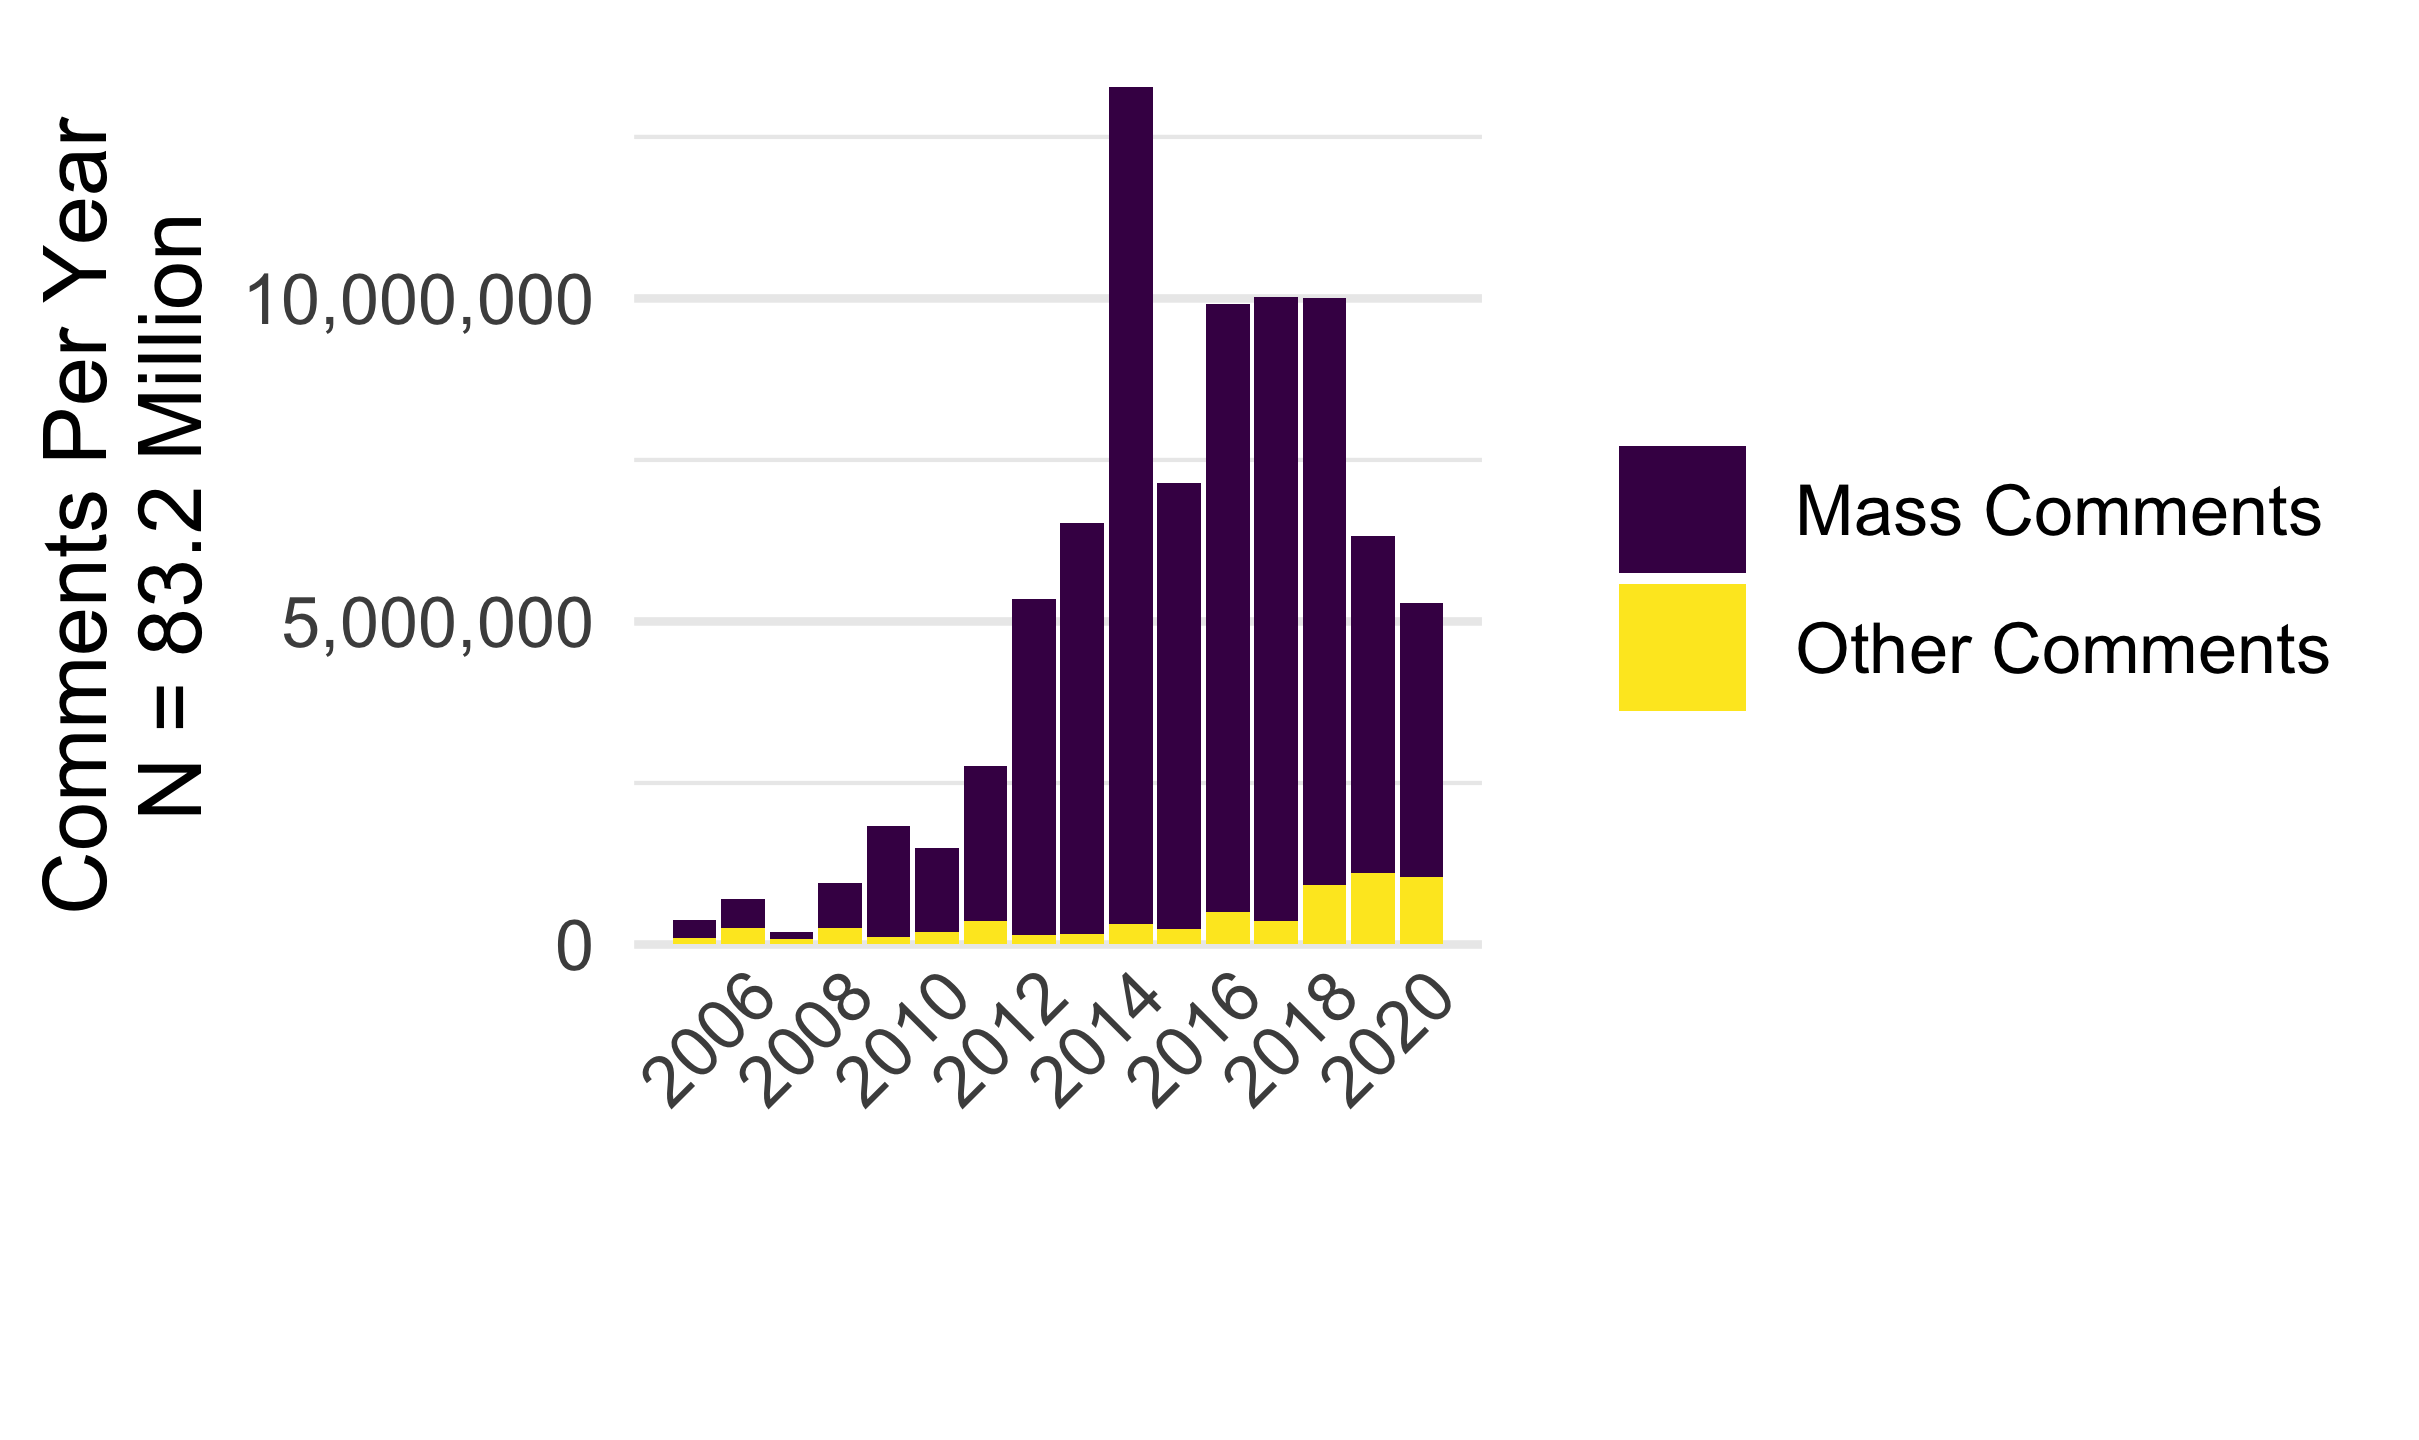
\includegraphics[height =2in]{Figs/comments-mass-1.png}
    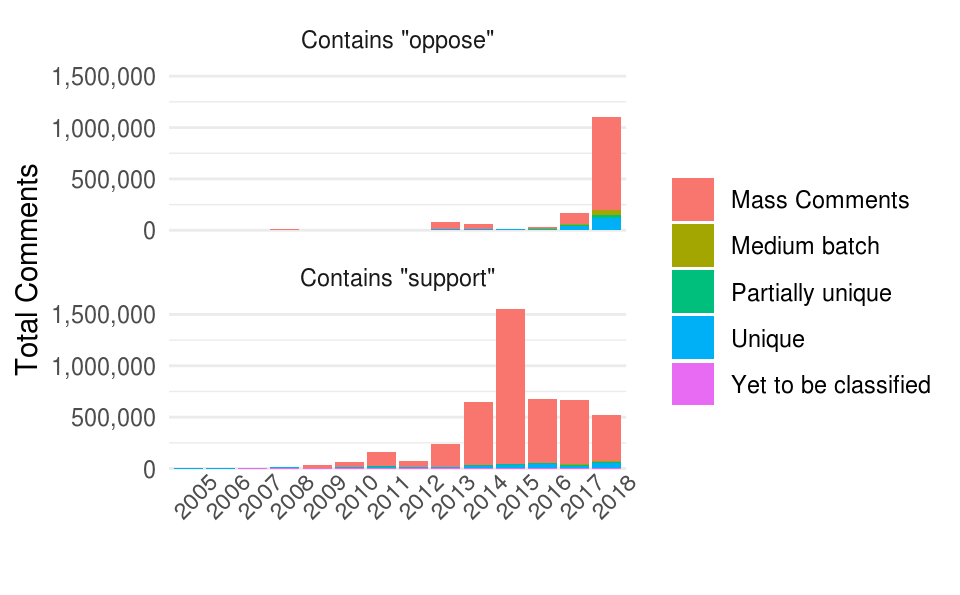
\includegraphics[height =2in]{Figs/comments-mass-support-vs-oppose-1.png}

    \label{fig:comments-support}
\end{figure}

The right pane of Figure \ref{fig:comments-support} shows results from a sample of several million comments for which I have digitized texts. Many of these comments appear to support proposed agency rules, as was the case with both the do not call and mercury rule examples. A rough measure of support (whether the comment text includes `` support '' or `` oppose '') shows that many more comments mention support, until 2018, when there is a fairly dramatic reversal in the share of comments mentioning ``support '' compared to those mentioning ``oppose '' (Figure \ref{fig:comments-support}). This may be a function of the changing regulatory agenda due to the change in presidential administration. 



\paragraph{Most comments occur on a small number of salient rules.} Approximately a third of public comments posted to regulations.gov were received on just ten regulations shown in figure \ref{fig:topdockets}.


\begin{figure}[h!]
    \centering
        \caption{Top 10 Dockets Receiving the Most Comments on regulations.gov and the top 20 Mobilizers}
    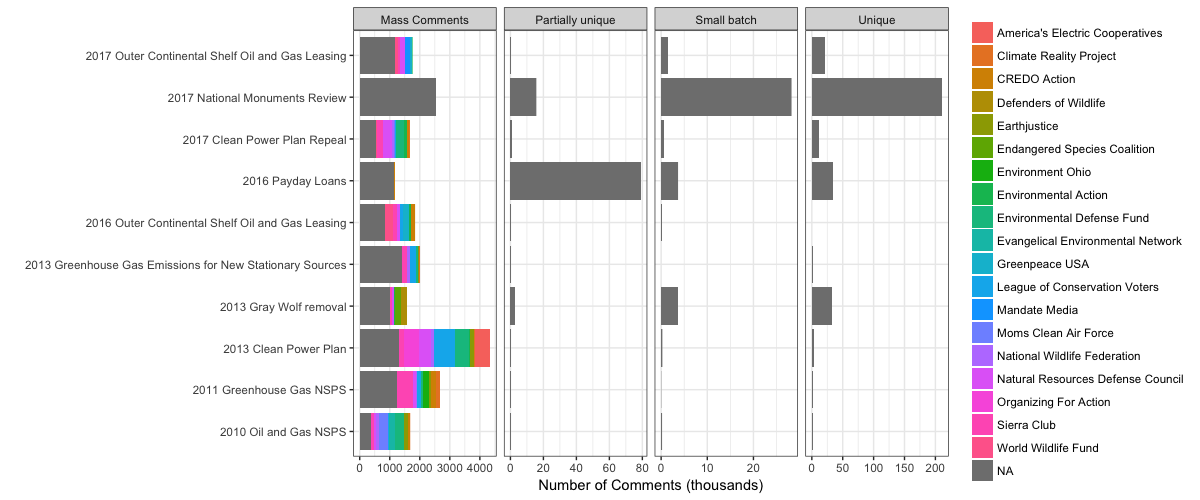
\includegraphics[width = 6in]{Figs/topdockets.png}
    \label{fig:topdockets}
\end{figure}


\paragraph{A coalition of public-interest organizations mobilize most comments.} As Figure \ref{fig:topdockets} % and \ref{fig:toporgs} 
shows, the most prolific mobilizers are environmental groups. On 5 out of the top 10 dockets (here including rulemaking and non-rulemaking dockets), a similar coalition of groups mobilized the majority of public comments. In part, this is because the Environmental Protection Agency produces a large share of the substantive rules posted to regulations.gov. However, it is notable that, on the top ten dockets, 19 of the top 20 mobilizers generally lobby together. America's Energy Cooperatives, an industry association, stands out as the lone mobilizer on behalf of material interest for its members. Notably, it only mobilized significantly on the Clean Power Plan but not on the subsequent Clean Power Plan repeal. 

\section{Conclusion}


% CONCLUSION
%This research will add to our understanding of how  bureaucratic policymaking fits with the practice of democracy.
%If input solicited from ordinary people has little effect on policy outcomes, directly or indirectly, it may be best understood as providing a veneer of democratic legitimacy on an essentially technocratic and/or elite-driven process.
The legitimacy of bureaucratic policymaking is said to depend on the premise that rulemaking provides for public voice \citep{Croley2003, Rosenbloom2003}. Yet we lack an empirical base necessary to evaluate whether any legitimacy the public comment process may provide is deserved. I have made a few initial steps toward better understanding actual public engagement in bureaucratic policymaking.
If mass engagement does shape agency decisions, a new research program will be needed to investigate who exactly these campaigns mobilize and represent.



\newpage
\section*{Appendix}


\begin{figure}[h!]
    \centering
        \caption{Rules ranked by number of comments posted to regulations.gov}
    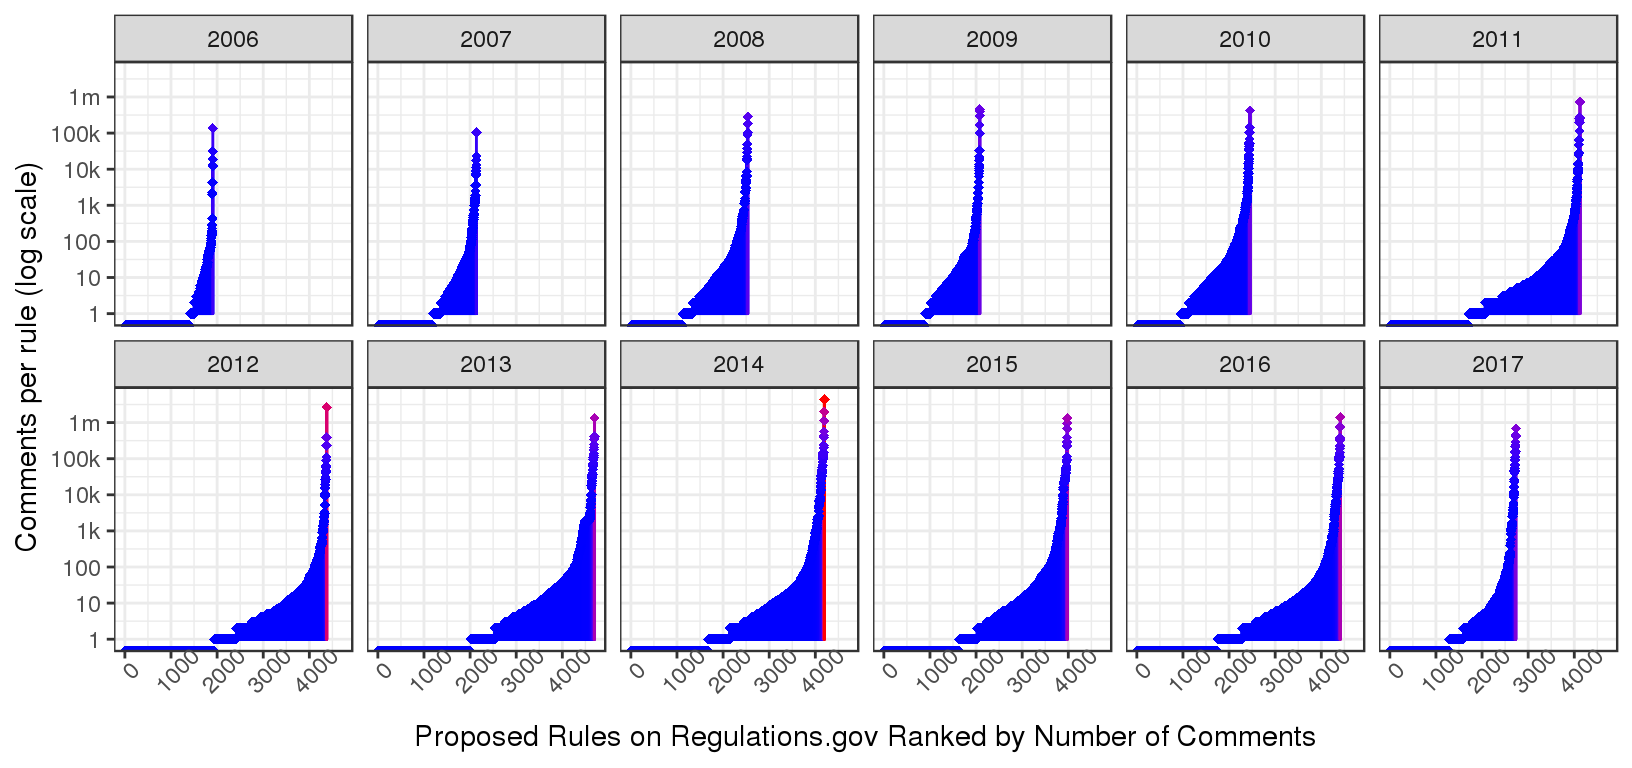
\includegraphics[width = 6.5in]{Figs/rules-ranked-comments-per-year-1.png}
    \label{fig:rules-ranked}
\end{figure}

\begin{figure}[p!]
    \centering
        \caption{Major and non-major rules on regulations.gov}
    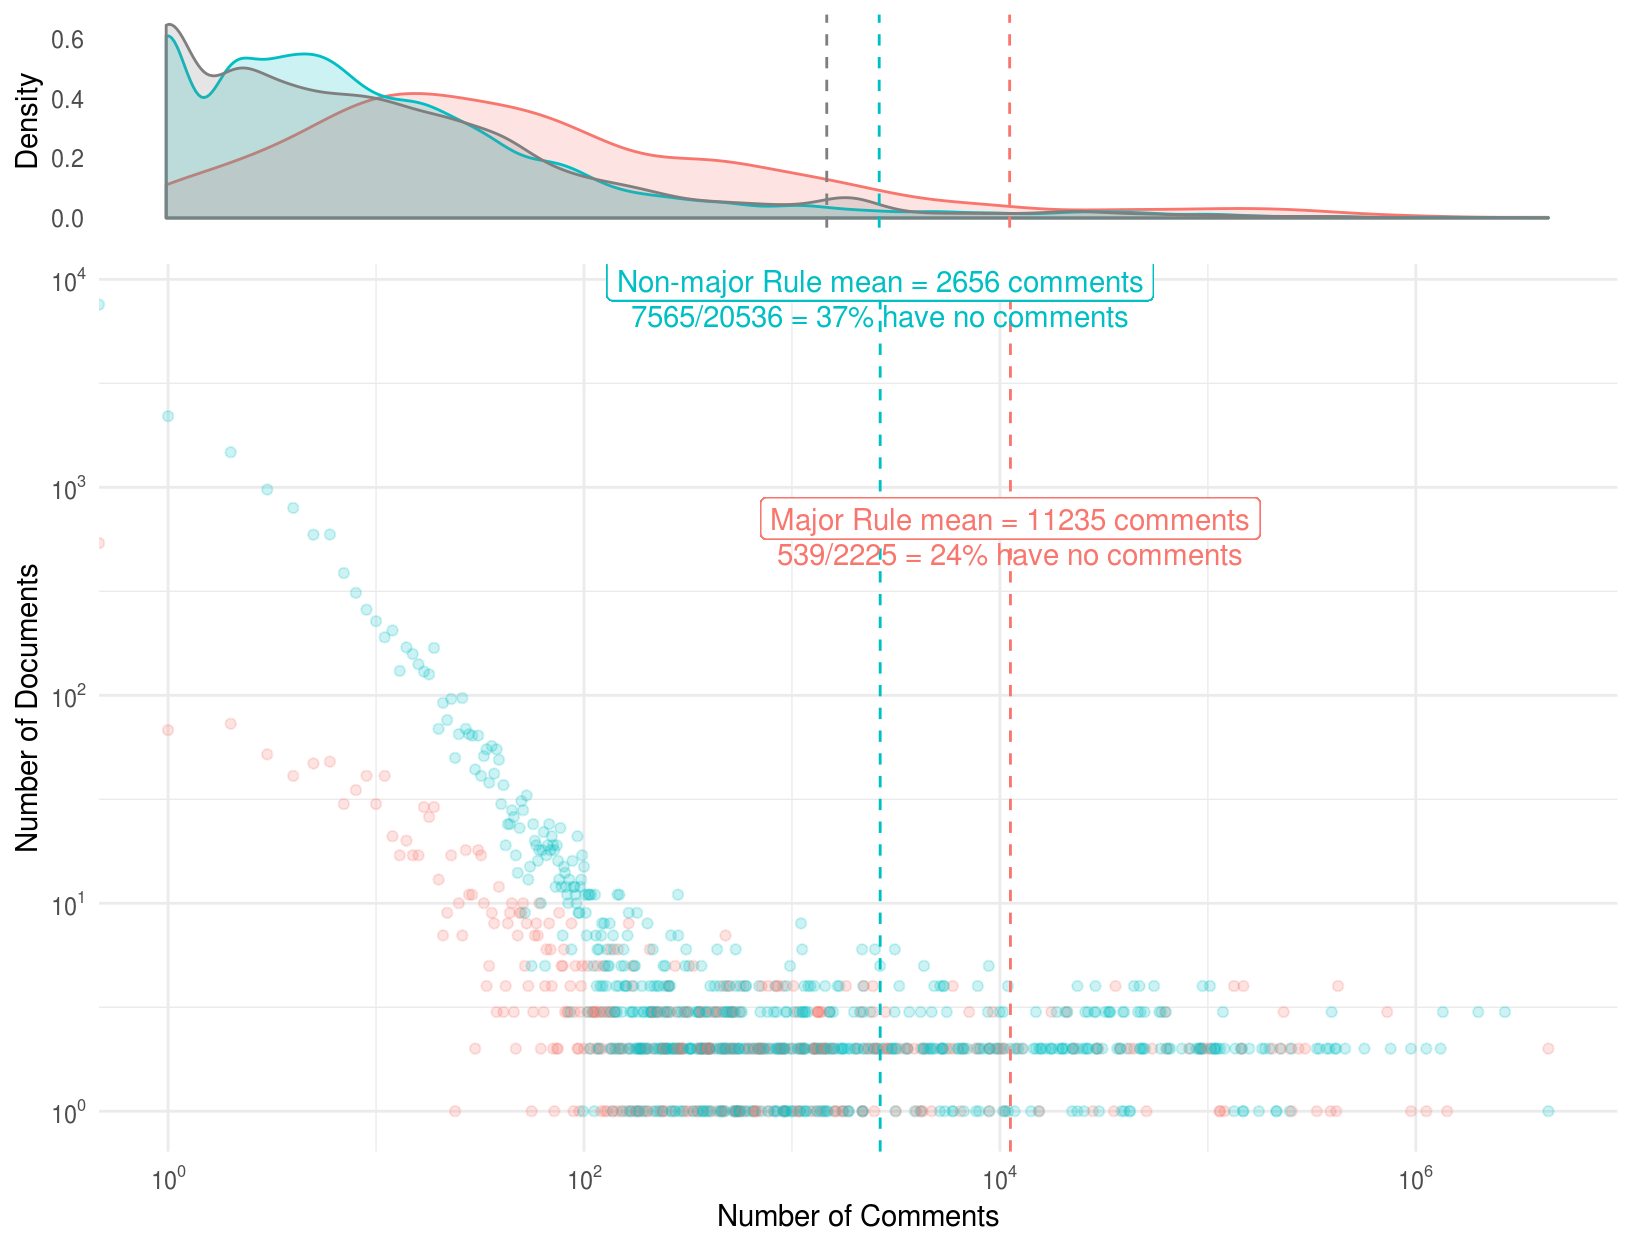
\includegraphics[width = 7in]{Figs/major-comments-density-1.png}
    \label{fig:rules-major}
\end{figure}

\begin{figure}[p!]
    \centering
        \caption{Rules on regulations.gov by priority level}
    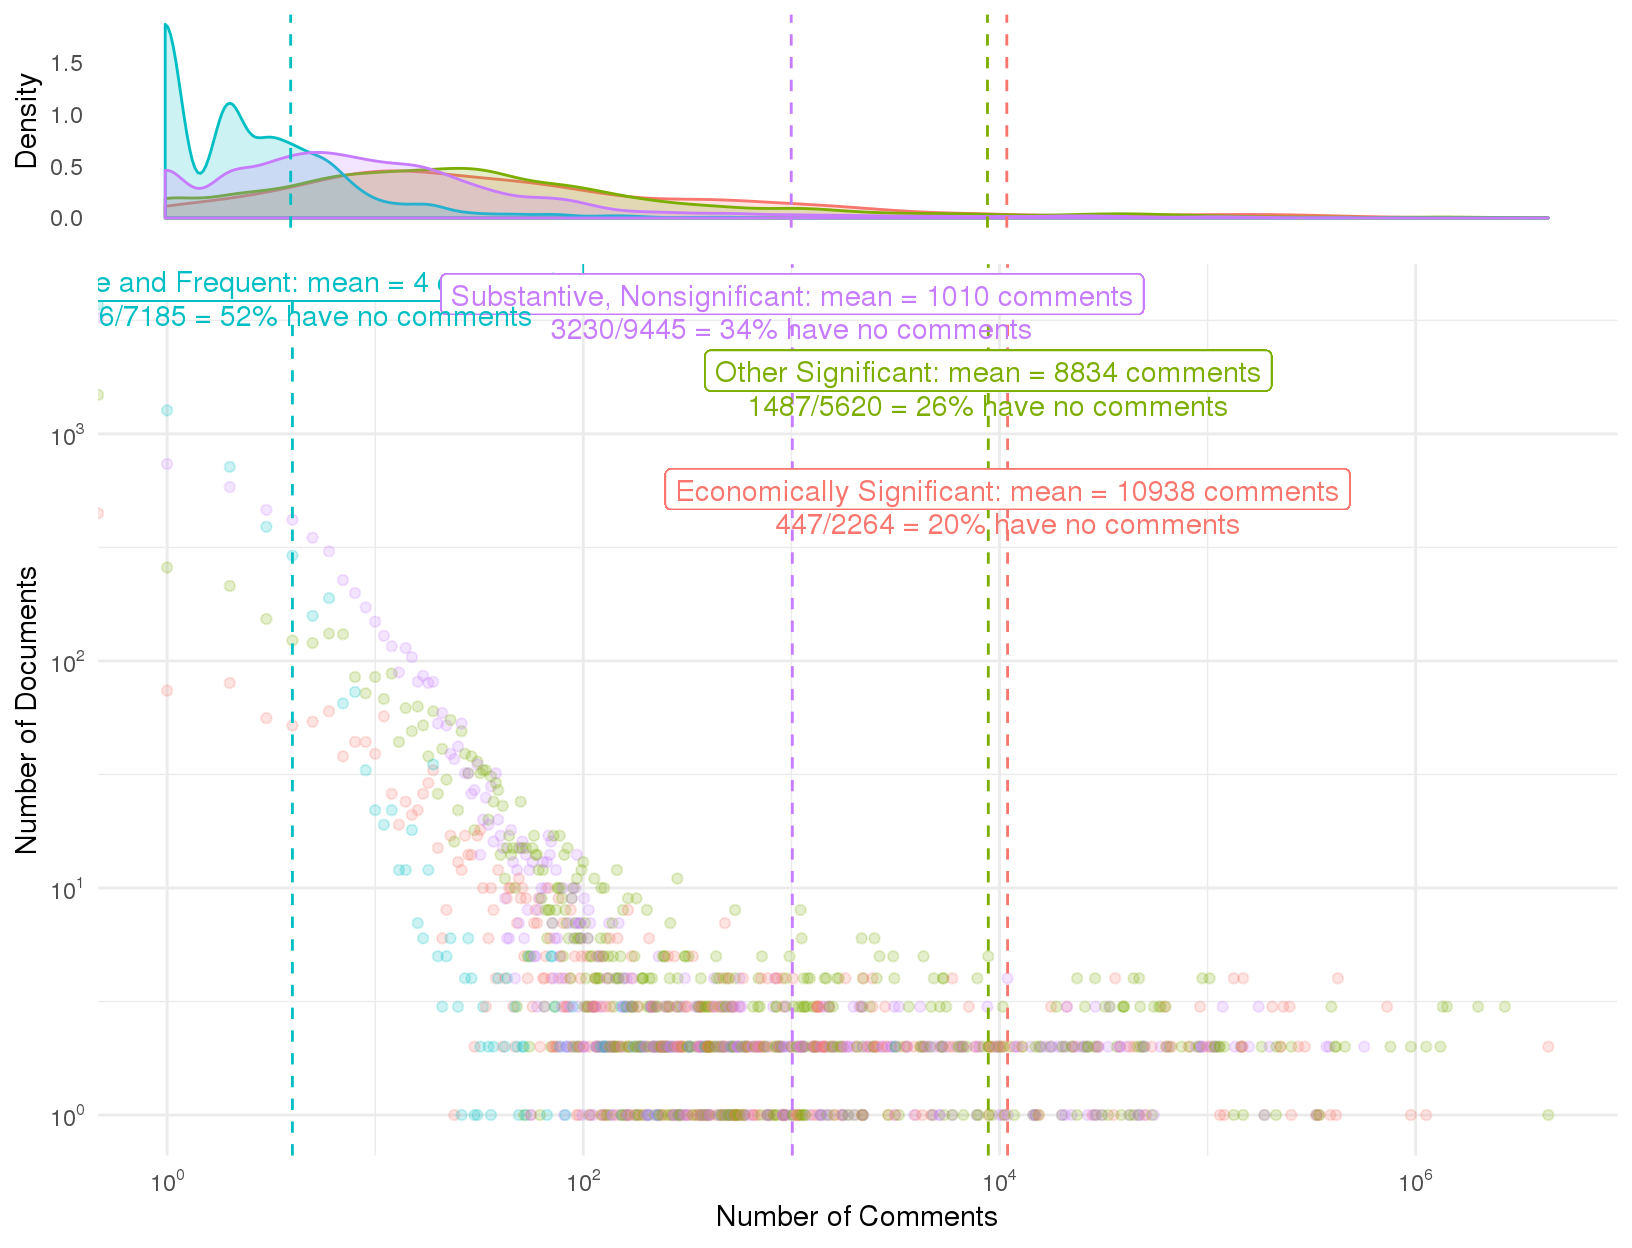
\includegraphics[width = 7in]{Figs/priority-comment-density-1.png}
    \label{fig:rules-priority}
\end{figure}

% FULL CAUSAL
\begin{figure}[h!]
    \centering
    \caption{The Role of Mass Commenting and Political Information in Bureaucratic Policymaking}
    \label{fig:causal-full}
\tiny
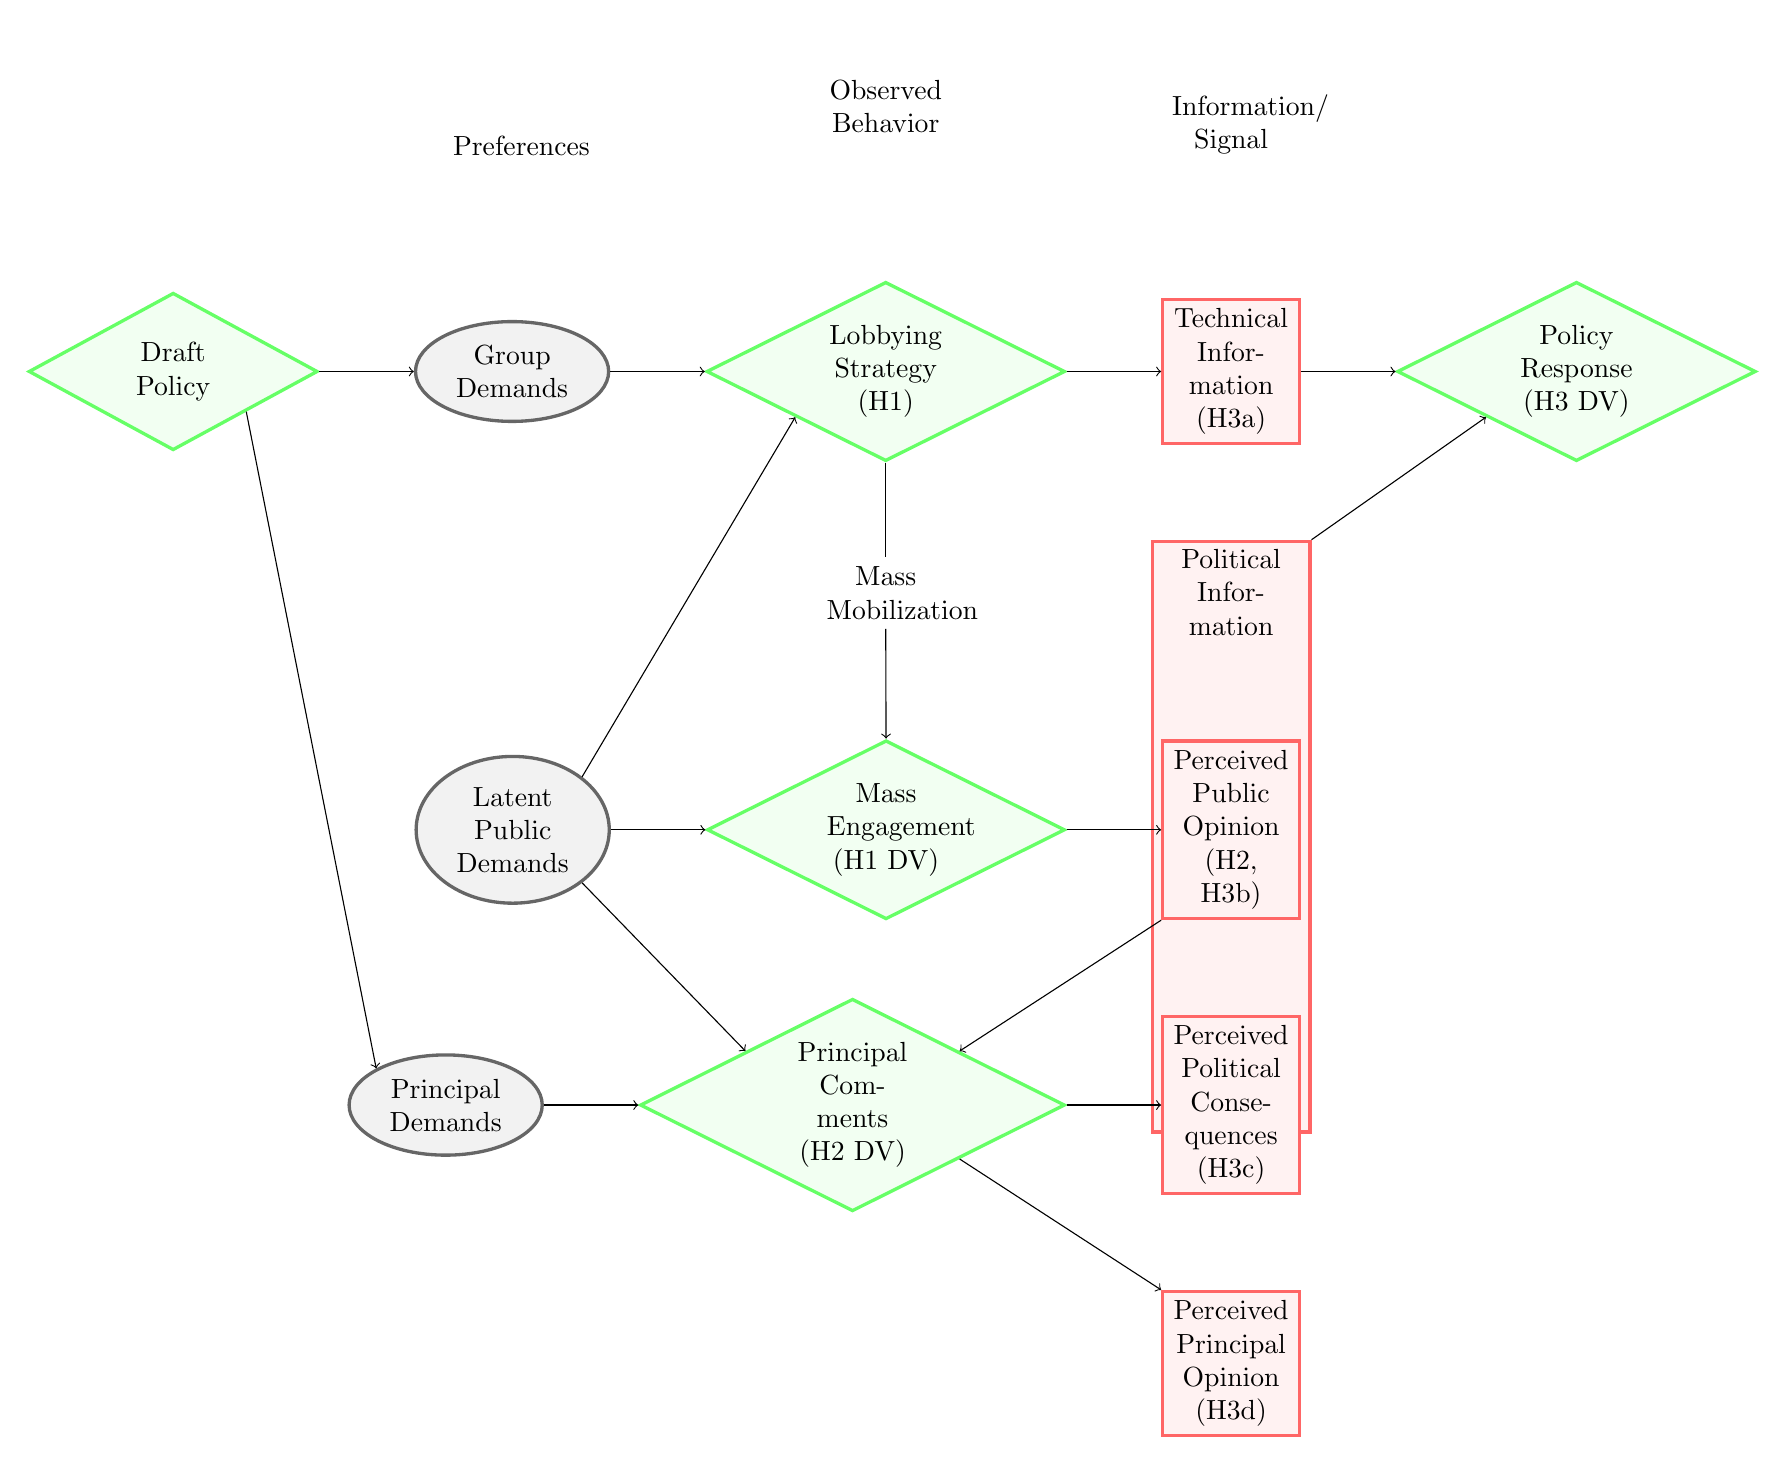
\begin{tikzpicture}[%
    node distance=1.2cm,
    auto,
    text width=1.5cm,
dnode/.style={diamond, align=center, aspect=2, fill=green!5,draw=green!60, very thick, minimum size=2cm},
squarednode/.style={rectangle, align=center, aspect=1, draw=red!60, fill=red!5, very thick, minimum size=1cm},
pnode/.style={ellipse, align=center, aspect=1, draw=black!60, fill=black!5, very thick, minimum size=1cm},
title/.style={rectangle, align=center, aspect=1, minimum size=2cm}
]
% Draft 
\node[dnode]      (draft)                     {Draft Policy};



% Group Nodes
\node[pnode]      (groupdemands) [right=of draft] {Group Demands};
\node[dnode]        (groupdecides) [right=of groupdemands] {Lobbying Strategy\\(H1)};
\node[squarednode]      (groupinfo) [right=of groupdecides] {Technical Information (H3a)};

% policy 
\node[dnode]      (policy)       [right=of groupinfo] {Policy Response\\(H3 DV)};
\draw[->] (groupinfo.east) -- (policy.west);
% \draw[->] (publicinfo.east) -- (policy.west);
% \draw[->] (principalinfo.east) -- (policy.south);
% \draw[->] (principalinfo2.east) -- (policy.south);

% Group Lines
\draw[->] (draft.east) -- (groupdemands.west);
\draw[->] (groupdemands.east) -- (groupdecides.west);
\draw[->] (groupdecides.east) -- (groupinfo.west);

% Titles
% \node[title]      (1) [above=of draft] {Policy};
\node[title]      (2) [above=of groupdemands] {Preferences};
\node[title]      (4) [above=of groupinfo] {Information/ Signal};
\node[title]      (3) [above=of groupdecides] {Observed Behavior};
% \node[title]      (5) [above=of policy] {Policy'};

% political info
\node[rectangle, minimum width =2cm, minimum height = 7.5cm, draw=red!60, fill=red!5, very thick]      (politicalinfo) [below=of groupinfo] {};
\node[text centered]      (politicalinfotext) [below=of groupinfo] {Political Information};
\node[text centered]      (mobilizing) [below=of groupdecides] {Mass\\ Mobilization};
\draw[->] (politicalinfo.north east) -- (policy.south west);

% public Nodes
\node[squarednode]      (publicinfo) [below=of politicalinfotext] {Perceived Public Opinion\\(H2, H3b)};
\node[dnode]      (publicdecides) [left=of publicinfo] {Mass\\ Engagement\\(H1 DV)};
\node[pnode]        (publicdemands) [left=of publicdecides] {Latent Public Demands};

% public Lines
% \draw[->] (draft.east) -- (publicdemands.west);
\draw[->] (publicdemands.east) -- (publicdecides.west);
\draw[->] (publicdemands.north east) -- (groupdecides.south west);
\draw[-] (groupdecides.south) -- (mobilizing.north);
\draw[->] (mobilizing.south) -- (publicdecides.north);
\draw[->] (publicdecides.east) -- (publicinfo.west);


% principal Nodes
\node[squarednode]      (principalinfo) [below=of publicinfo] {Perceived Political Consequences\\(H3c)};
\node[dnode]      (principaldecides) [left=of principalinfo] {Principal Comments\\(H2 DV)};
\node[pnode]        (principaldemands) [left=of principaldecides] {Principal Demands};
\node[squarednode]      (principalinfo2) [below=of principalinfo] {Perceived Principal Opinion\\(H3d)};


% principal Lines
\draw[->] (draft.south east) -- (principaldemands.north west);
\draw[->] (principaldemands.east) -- (principaldecides.west);
\draw[->] (publicinfo.south west) -- (principaldecides.north east);
\draw[->] (principaldecides.east) -- (principalinfo.west);
\draw[->] (principaldecides.south east) -- (principalinfo2.north west);
\draw[->] (publicdemands.south east) -- (principaldecides.north west);

\end{tikzpicture}
\end{figure}
\normalsize


\clearpage 



%\theendnotes
\singlespace
\small
\bibliographystyle{apsr.bst} 
\bibliography{mendeley.bib}
\end{document}

